% !TEX encoding = UTF-8
% !TEX TS-program = pdflatex
% !TEX root = ../testex
% !TEX spellcheck = it-IT

%**************************************************************
\chapter{XML Editor}
\label{cap:xml-editor}
%**************************************************************

\intro{In questo capitolo è presente una analisi completa del tool XML Editor}\\

\section{Introduzione}

	\subsection{Premessa}
		L'engine di un videogioco, se sviluppato secondo una buona architettura, legge da file di configurazione la maggior parte delle informazioni piuttosto di averle scritte direttamente nel codice\footnote{La pratica di scrivere nel gioco le informazioni è comunemente chiamata \textit{Hard-coding}.}. I file di configurazione possono essere poi specializzati per una specifica piattaforma come già visto nel \nameref{cap:multiplatform-file-analyzer}. Il contenuto di questi file può essere estremamente vario, ad esempio sono utilizzati per indicare i percorsi delle pagine dei menu, la descrizione degli oggetti grafici in relazione alle sotto-componenti e alle animazioni. Gli standard prevedono che tali file di configurazione vengano scritti mediante il linguaggio XML.

	\subsection{Lo scopo}
		Vista l'eterogeneità dei file di configurazione ed del team di sviluppo di un gioco, è possibile che questi siano scritti anche da persone non specializzate (esempio: artisti). Inoltre, è possibile inserire relazioni tra elementi presenti in questi file. Ad esempio, per un oggetto grafico si specifica quali sono gli oggetti attaccati allo scheletro di animazione, elementi che sono definiti solitamente in un altro file di configurazione. Essendo questi caricati a run-time, il debugging diviene decisamente non banale, in quanto non è semplice capire da dove l'errore proviene essendo moltissime le variabili in gioco.\\
		
		Il tool si pone l'obbiettivo di rendere la scrittura e il debugging dei file di configurazione XML più semplice e veloce. Innanzitutto fornirà un editor visuale in cui sarà possibile editare in tutti gli aspetti l'XML. Verrà inoltre fornita la possibilità di specificare le relazioni ed eventuali altri file coinvolti, dopodiché il programma sarà in grado di verificare le relazioni nei file aperti e di crearne di nuove tramite un semplice drag \& drop dei nodi destinatari della relazione.

\section{Casi d'uso}

	Per meglio capire e tracciare l'esperienza d'uso che un developer di un gioco avrà con il tool sono stati creati dei diagrammi di casi d'uso gerarchici.\\
	I diagrammi di casi d'uso fanno parte della famiglia dei diagrammi UML e descrivono le funzionalità offerte dal prodotto così come sono percepite dagli attore che interagiscono con il sistema.\\
	Ogni caso d'uso ha un codice univoco gerarchico, nella forma:
	\begin{center} 
		UC[codice univoco del padre].[codice progressivo di livello]
	\end{center}
	\paragrafo Il codice progressivo può includere diversi livelli di gerarchia separati da un punto.

	\subsection{UC 1: Caso d'uso principale}
		\label{subsec:XEUC1}
		
		\begin{figure}[!h] 
			\centering 
			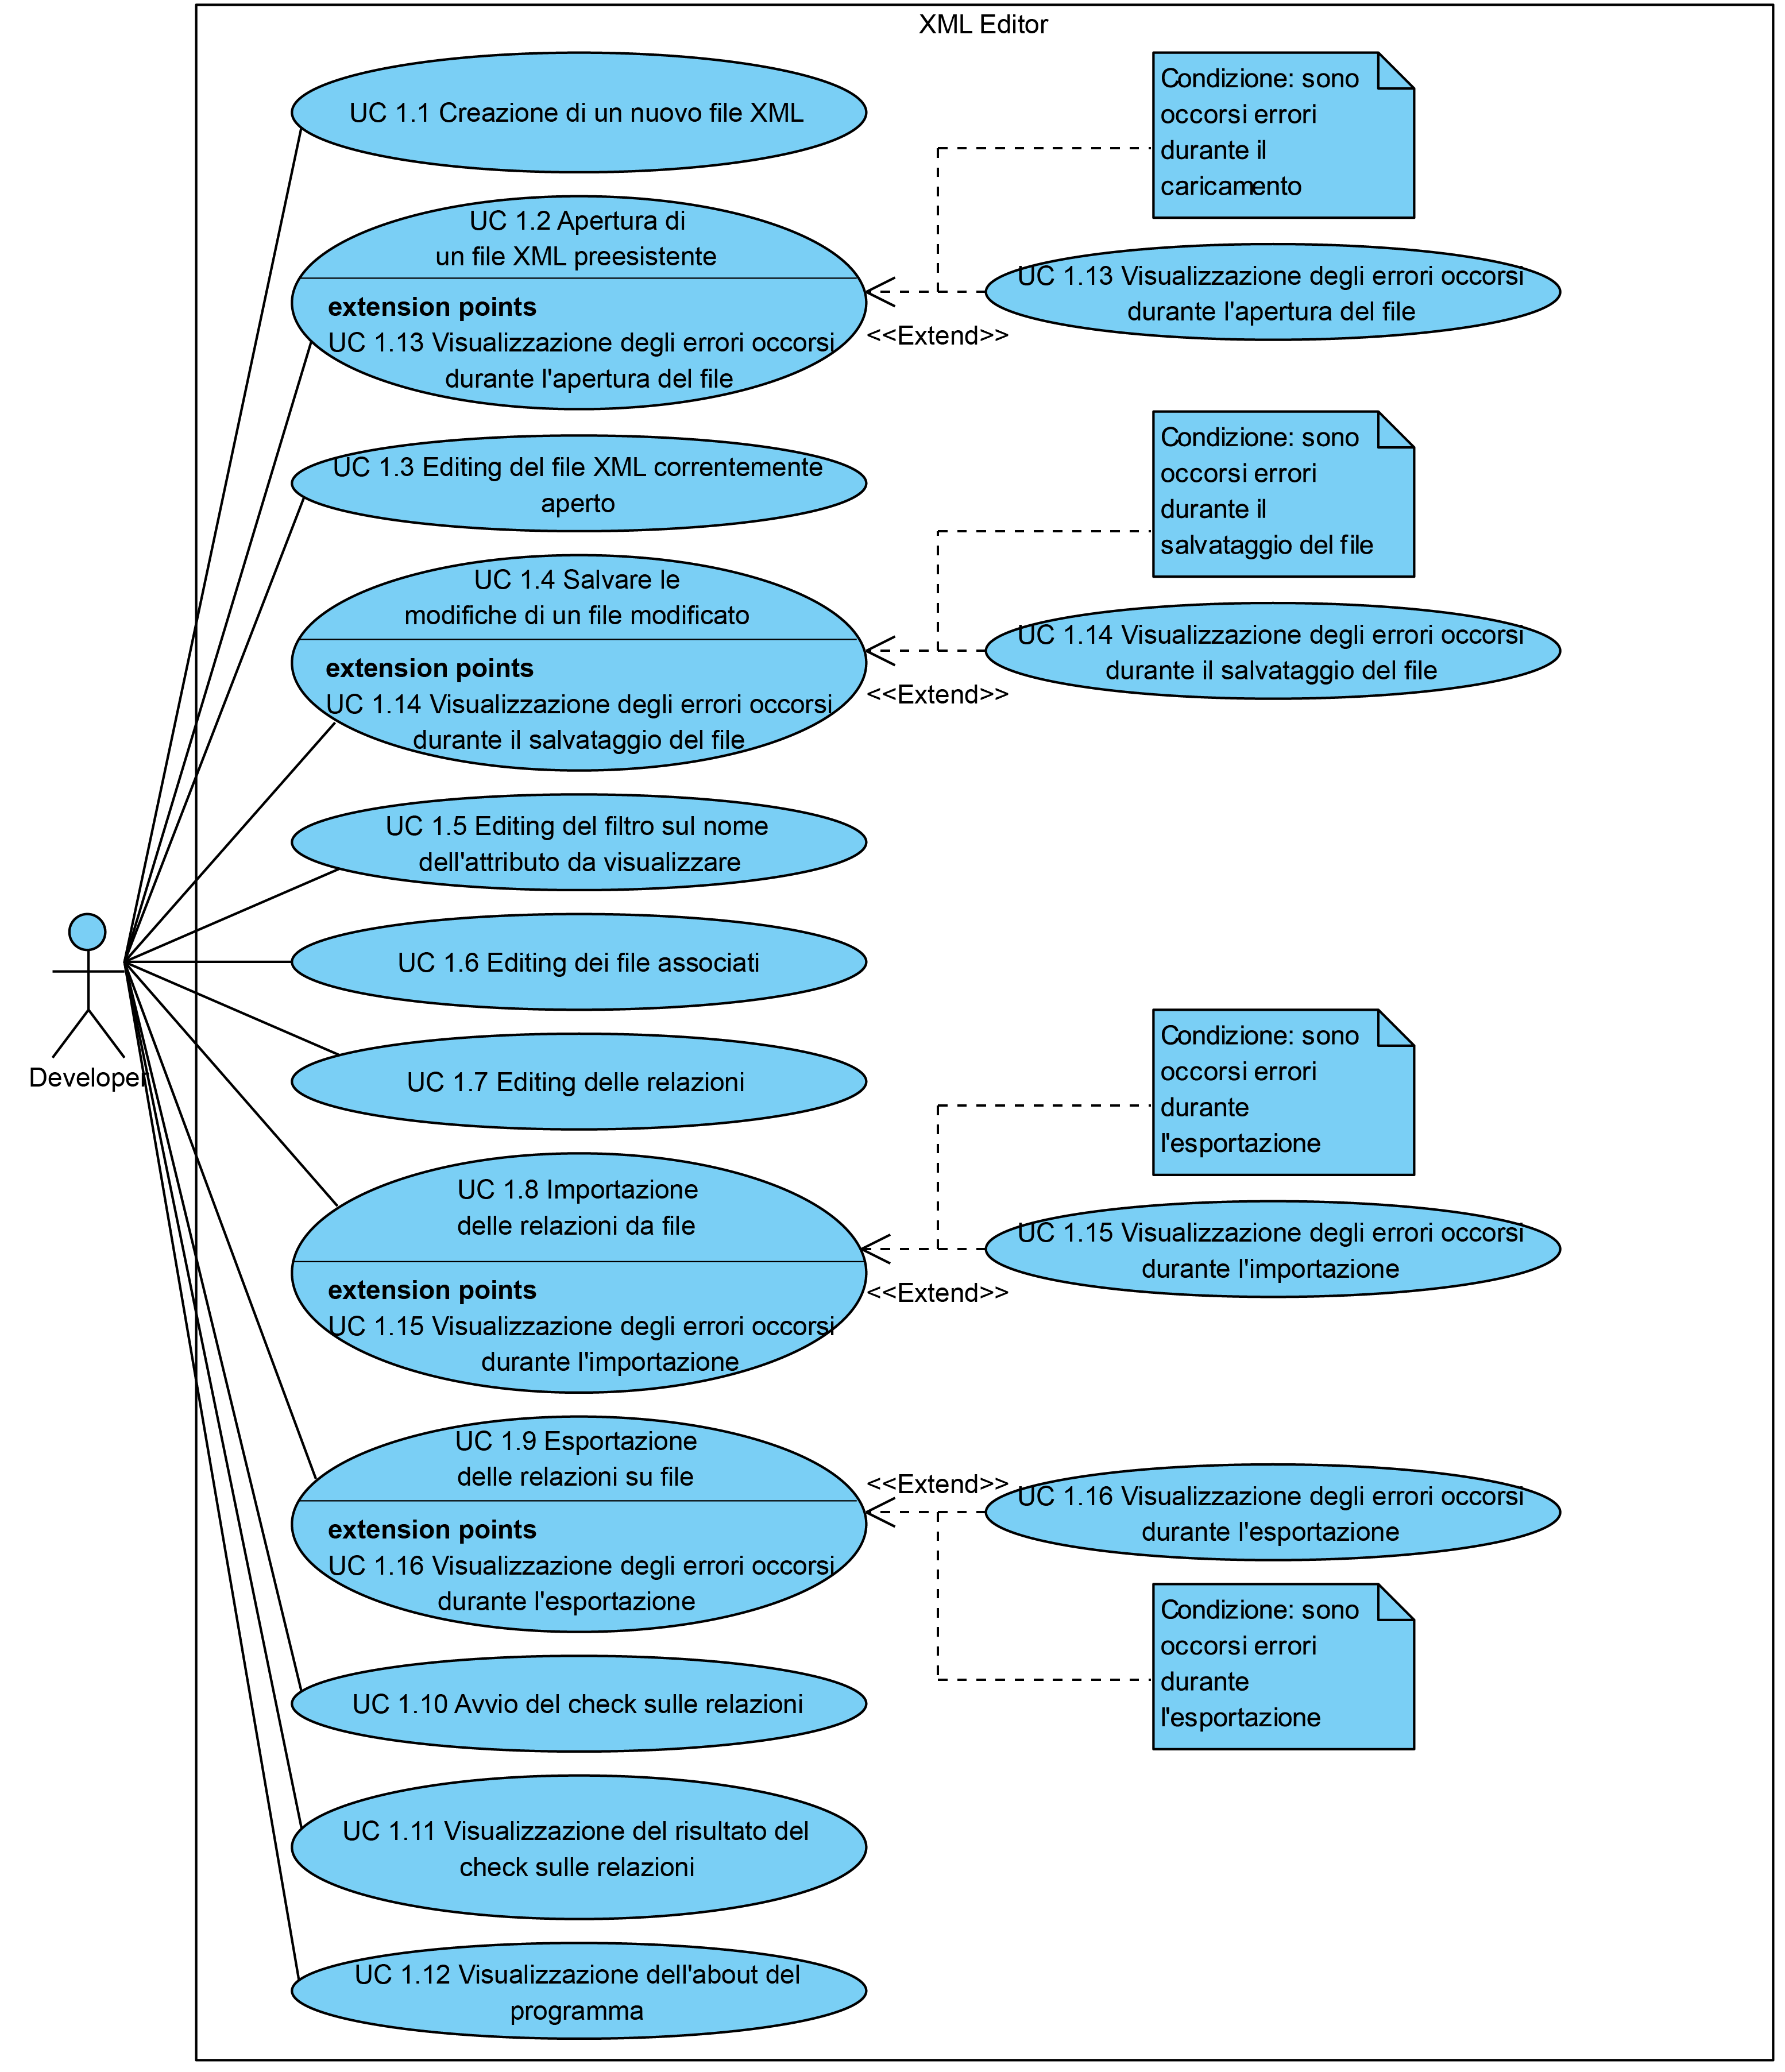
\includegraphics[width=0.9\columnwidth]{tool2/UC1.png} 
			\caption{Use Case - UC 1: Caso d'uso principale}
		\end{figure}
		
		\begin{itemize}
			\item\textbf{Attori}: developer.
			\item\textbf{Descrizione}: un developer deve avere tutte le funzionalità a disposizione per editare ed verificare uno o più file XML.
			\item\textbf{Precondizione}: il developer abbia lanciato il tool sotto un sistema Windows 7 o superiore.
			\item\textbf{Flusso principale degli eventi}: 
			\begin{enumerate}
				\item \textit{l'utente ha la possibilità di:} \textit{creazione di un nuovo file XML} (\hyperref[subsec:XEUC1.1]{UC 1.1});
				
				\item \textit{l'utente ha la possibilità di:} \textit{apertura di un file XML preesistente} (\hyperref[subsec:XEUC1.2]{UC 1.2});
				
				\item \textit{l'utente ha la possibilità di:} \textit{editing del file XML correntemente aperto} (\hyperref[subsec:XEUC1.3]{UC 1.3});
				
				\item \textit{l'utente ha la possibilità di:} \textit{salvare le modifiche di un file modificato} (\hyperref[subsec:XEUC1.4]{UC 1.4});
				
				\item \textit{l'utente ha la possibilità di:} \textit{editing del filtro sul nome dell'attributo da visualizzare} (\hyperref[subsec:XEUC1.5]{UC 1.5});
				
				\item \textit{l'utente ha la possibilità di:} \textit{editing dei file associati} (\hyperref[subsec:XEUC1.6]{UC 1.6});
				
				\item \textit{l'utente ha la possibilità di:} \textit{editing delle relazioni} (\hyperref[subsec:XEUC1.7]{UC 1.7});
				
				\item \textit{l'utente ha la possibilità di:} \textit{importazione delle relazioni da file} (\hyperref[subsec:XEUC1.8]{UC 1.8});
				
				\item \textit{l'utente ha la possibilità di:} \textit{esportazione delle relazioni su file} (\hyperref[subsec:XEUC1.9]{UC 1.9});
				
				\item \textit{l'utente ha la possibilità di:} \textit{avvio del check sulle relazioni} (\hyperref[subsec:XEUC1.10]{UC 1.10});
				
				\item \textit{l'utente ha la possibilità di:} \textit{visualizzazione del risultato del check sulle relazioni} (\hyperref[subsec:XEUC1.11]{UC 1.11});
				
				\item \textit{l'utente ha la possibilità di:} \textit{visualizzazione dell'about del programma} (\hyperref[subsec:XEUC1.12]{UC 1.12}).
				
			\end{enumerate}
			\item \textbf{Estensioni}
			\begin{enumerate}
				\item\textit{Visualizzazione degli errori occorsi durante l'apertura del file} (\hyperref[subsec:XEUC1.13]{UC 1.13});
				
				\item\textit{Visualizzazione degli errori occorsi durante il salvataggio del file} (\hyperref[subsec:XEUC1.14]{UC 1.14});
				
				\item\textit{Visualizzazione degli errori occorsi durante l'importazione} (\hyperref[subsec:XEUC1.15]{UC 1.15});
				
				\item\textit{Visualizzazione degli errori occorsi durante l'esportazione} (\hyperref[subsec:XEUC1.16]{UC 1.16}).
			\end{enumerate}
			\item\textbf{Postcondizione}: il sistema ha erogato le funzionalità richieste dal developer.
		\end{itemize}

	\subsection{UC 1.1: Creazione di un nuovo file XML}
		\label{subsec:XEUC1.1}
	
		\begin{figure}[!h] 
			\centering 
			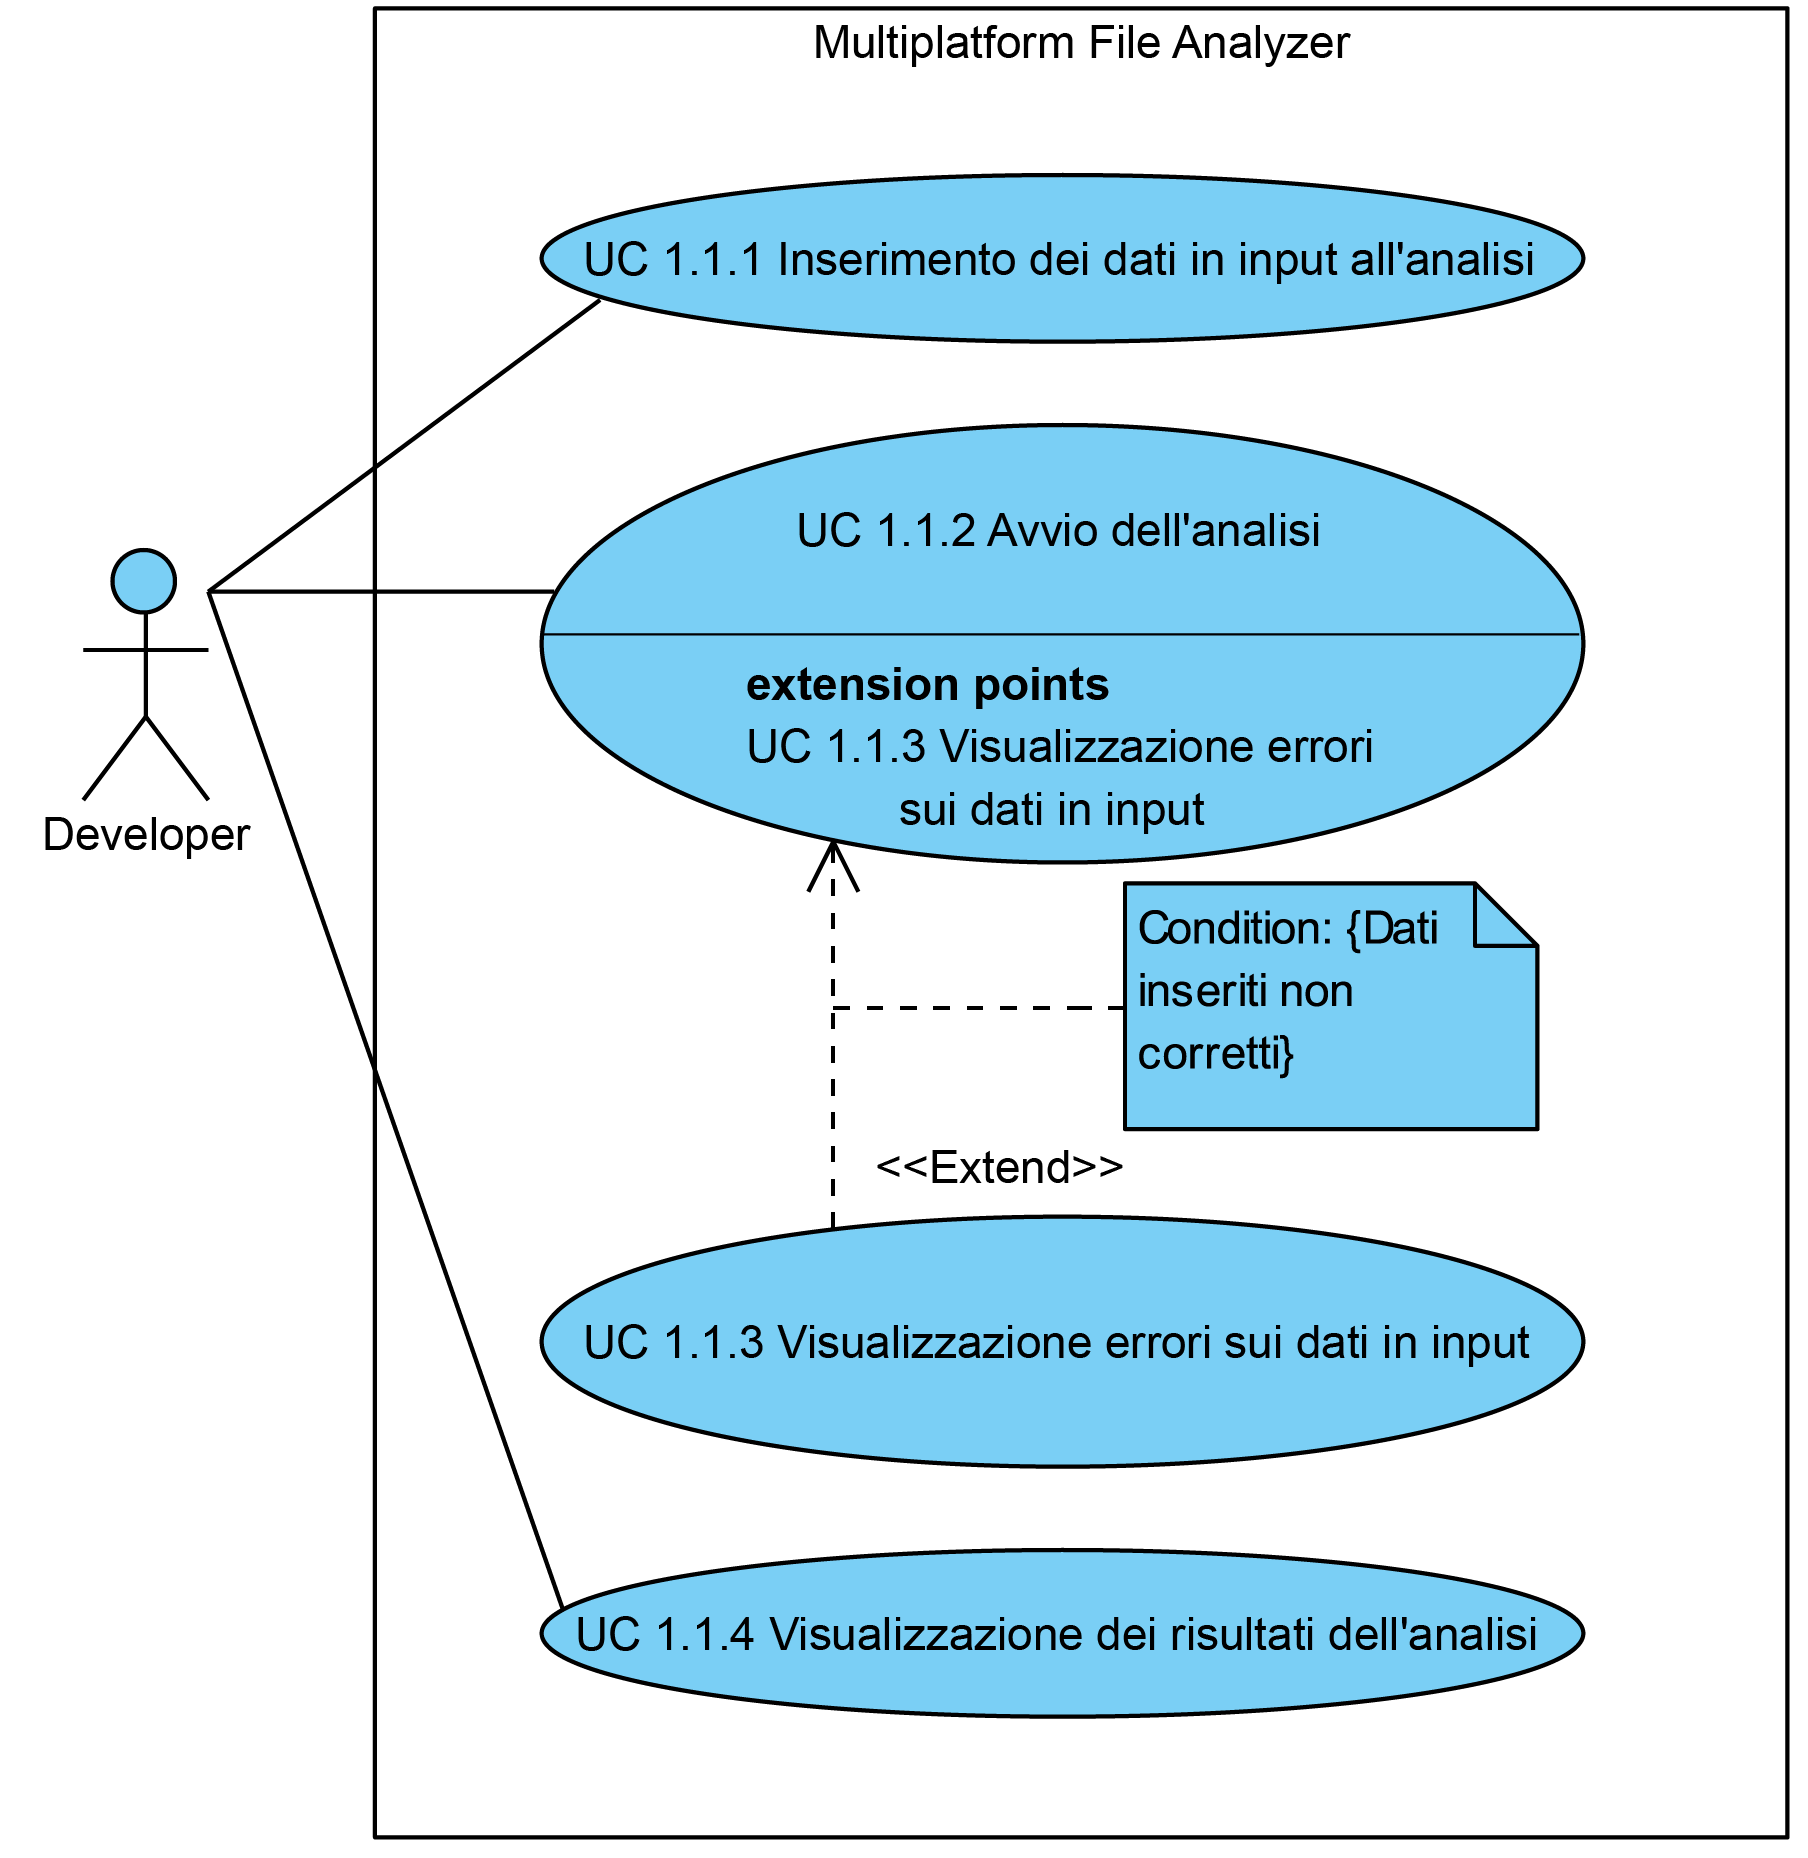
\includegraphics[width=0.9\columnwidth]{tool2/UC1-1.png} 
			\caption{Use Case - UC 1.1: Creazione di un nuovo file XML}
		\end{figure}
		
		\begin{itemize}
			\item\textbf{Attori}: developer.
			\item\textbf{Descrizione}: un developer deve poter creare un nuovo file XML.
			\item\textbf{Precondizione}: il developer ha lanciato il tool sotto un sistema Windows 7 o superiore.
			\item\textbf{Flusso principale degli eventi}: 
			\begin{enumerate}
				\item\textit{Inserimento del percorso dove memorizzare il nuovo XML} (\hyperref[subsec:XEUC1.1.1]{UC 1.1.1});
				\item\textit{Inserimento del nome del file del nuovo XML} (\hyperref[subsec:XEUC1.1.2]{UC 1.1.2}).
			\end{enumerate}
			\item\textbf{Postcondizione}: il sistema ha creato un nuovo file XML in memoria, esso sarà salvato su disco solo nel momento in cui l'utente lo salverà. Il sistema chiude il lavoro corrente e apre il nuovo file creato.
		\end{itemize}
		
	\subsection{UC 1.1.1: Inserimento del percorso dove memorizzare il nuovo XML}
		\label{subsec:XEUC1.1.1}
		
		\begin{itemize}
			\item\textbf{Attori}: developer.
			\item\textbf{Descrizione}: un developer deve poter inserire il percorso dove memorizzare su disco il nuovo file XML.
			\item\textbf{Precondizione}: il developer abbia selezionato l'azione per creare un nuovo file XML.
			\item\textbf{Scenario principale}: il developer sceglie il percorso dove memorizzare il nuovo file XML.
			\item\textbf{Postcondizione}: il sistema ha memorizzato il percorso dove salvare il nuovo file XML.
		\end{itemize}
		
	\subsection{UC 1.1.2: Inserimento del nome del file del nuovo XML}
		\label{subsec:XEUC1.1.2}
		
		\begin{itemize}
			\item\textbf{Attori}: developer.
			\item\textbf{Descrizione}: un developer deve poter inserire il nome del nuovo file XML.
			\item\textbf{Precondizione}: il developer abbia selezionato l'azione per creare un nuovo file XML.
			\item\textbf{Scenario principale}: il developer inserisce il nome del nuovo file XML.
			\item\textbf{Postcondizione}: il sistema ha memorizzato il nome del nuovo file XML.
		\end{itemize}
		
	\subsection{UC 1.2: Apertura di un file XML preesistente}
		\label{subsec:XEUC1.2}
		
		\begin{itemize}
			\item\textbf{Attori}: developer.
			\item\textbf{Descrizione}: un developer deve poter aprire un file XML preesistente.
			\item\textbf{Precondizione}: il developer abbia selezionato l'azione per aprire un file XML.
			\item\textbf{Scenario principale}: il developer inserisce il percorso ed il nome del file XML da aprire.
			\item\textbf{Postcondizione}: il sistema ha chiuso il lavoro precedentemente aperto e l'ha sostituito con il file XML selezionato. Se il file era stato precedentemente aperto ed erano stati settati alcuni file associati allora anche quei file saranno aperti.
		\end{itemize}
		
	\subsection{UC 1.3 Editing del file XML correntemente aperto}
		\label{subsec:XEUC1.3}
		
		\begin{figure}[!h] 
			\centering 
			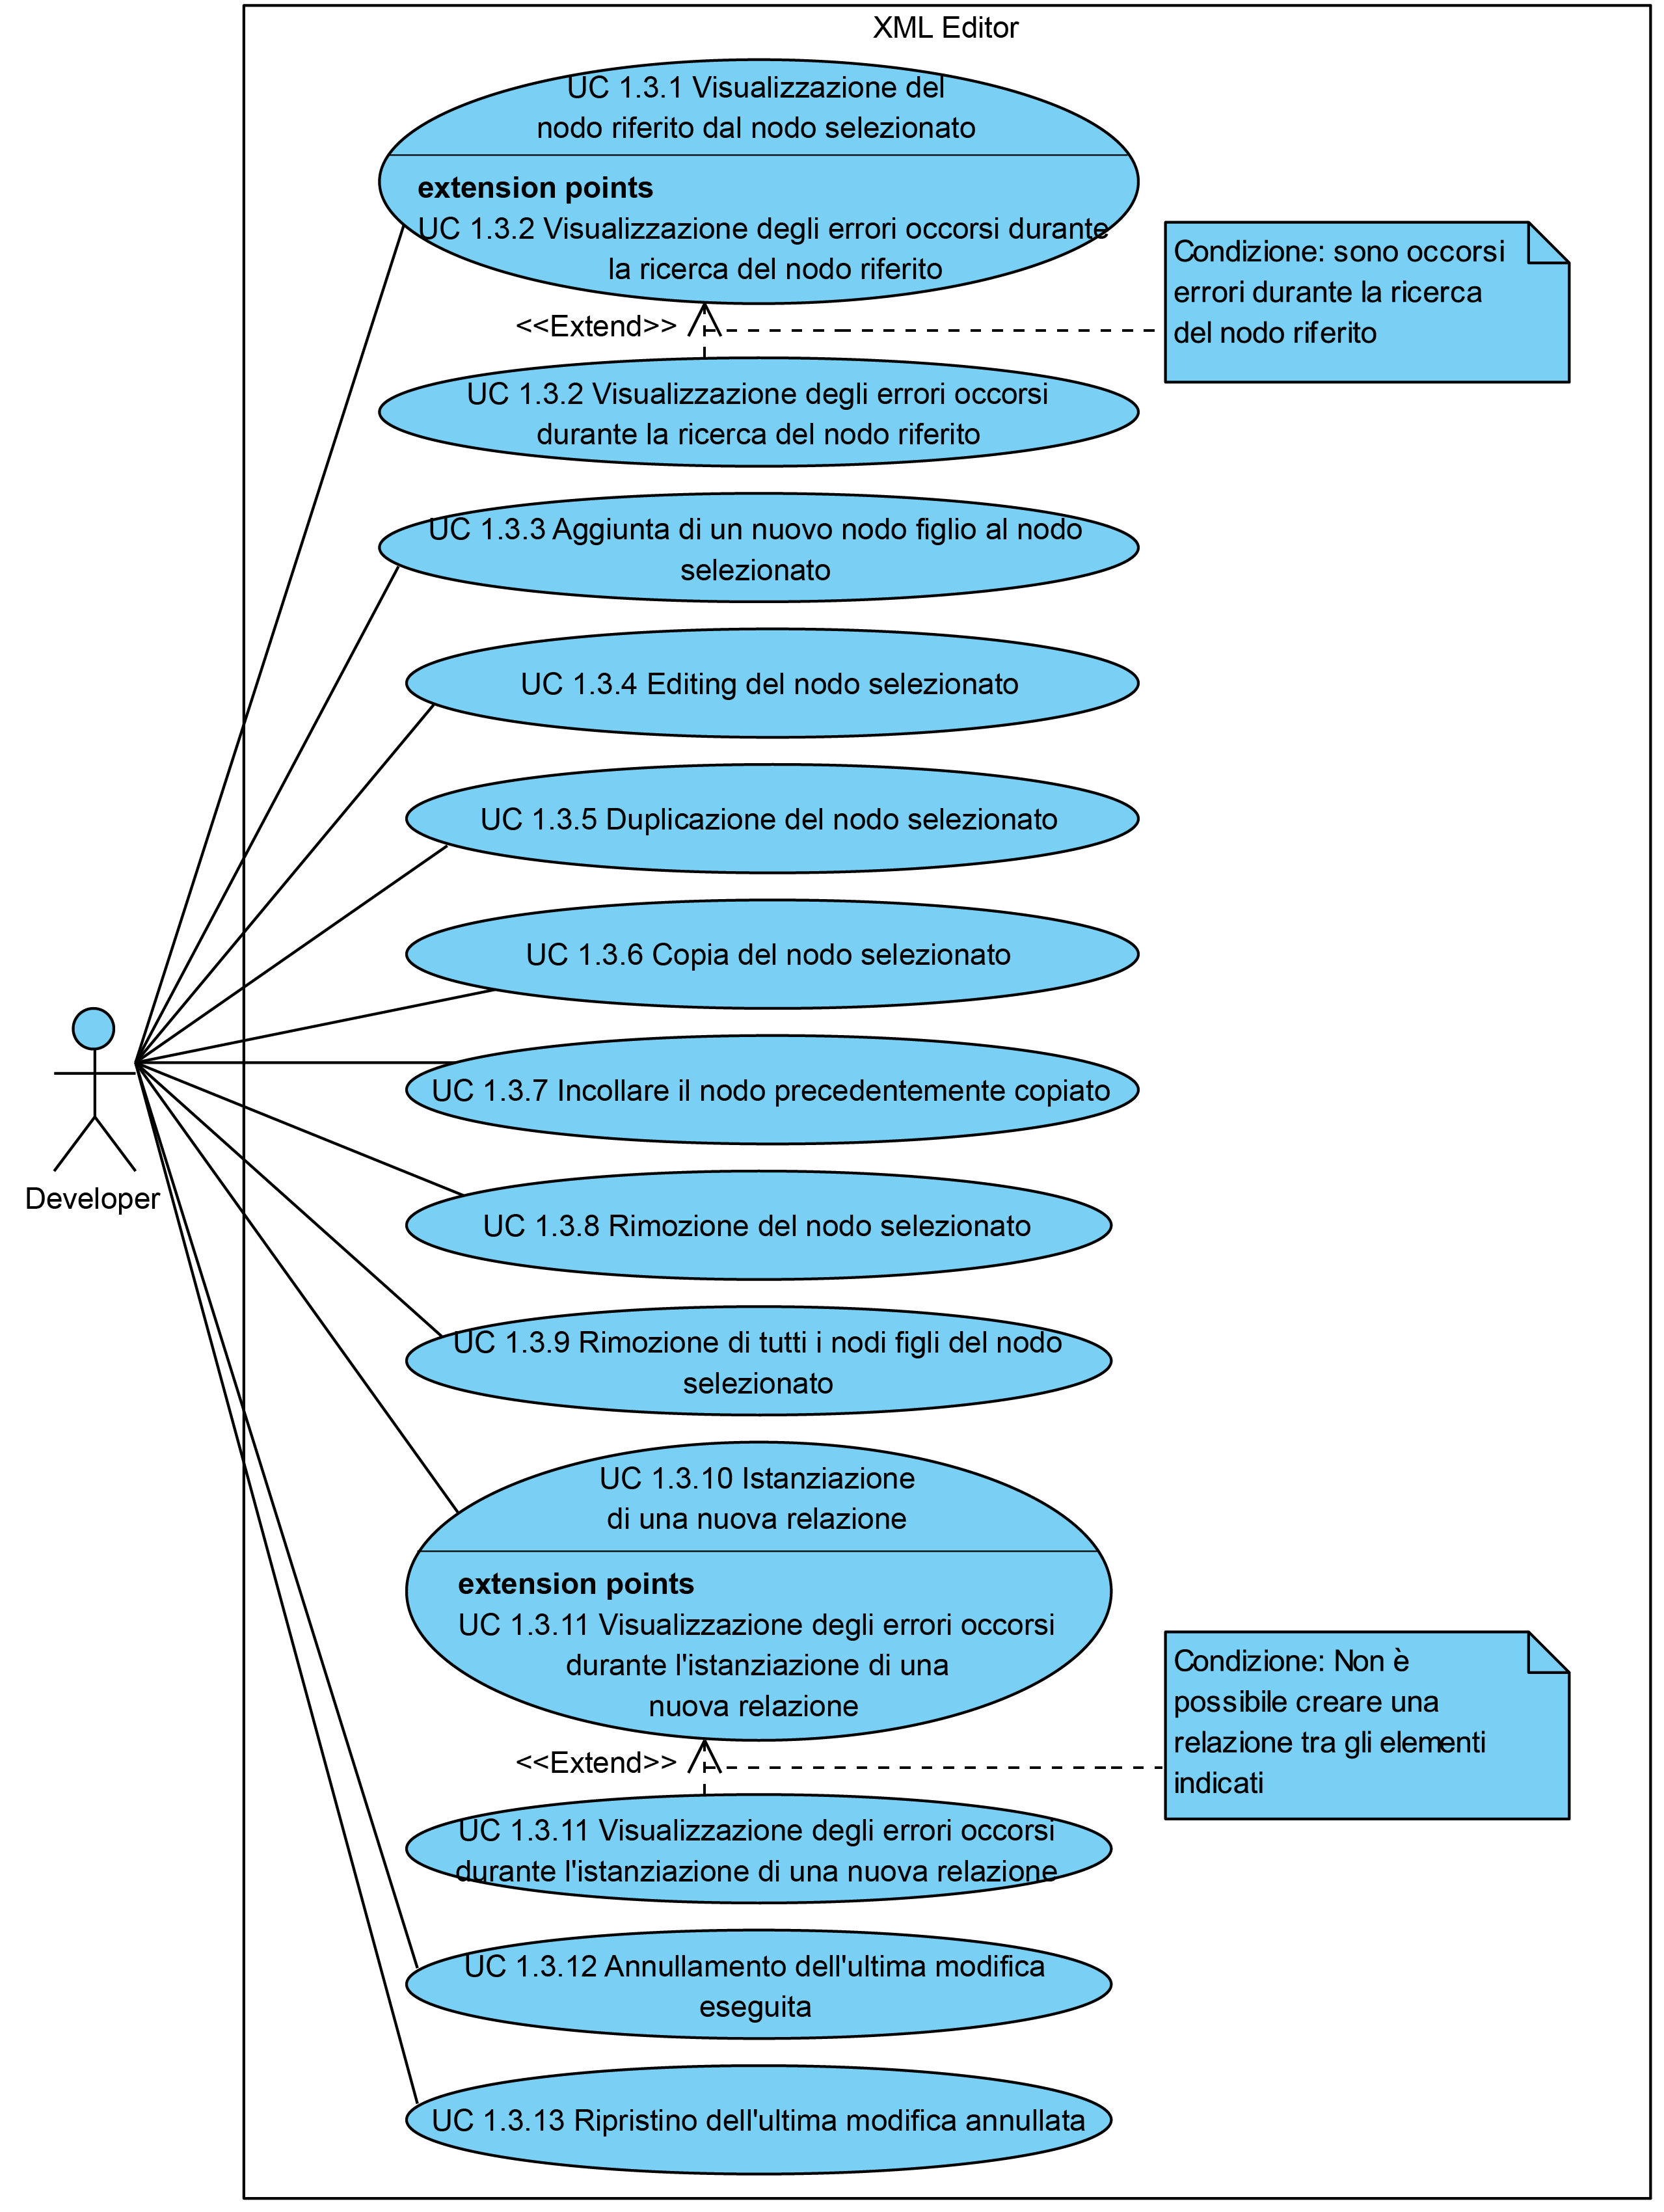
\includegraphics[width=0.9\columnwidth]{tool2/UC1-3.png} 
			\caption{Use Case - UC 1.3 Editing del file XML correntemente aperto}
		\end{figure}
		
		\begin{itemize}
			\item\textbf{Attori}: developer.
			\item\textbf{Descrizione}: un developer deve poter editare il file XML correntemente visualizzato.
			\item\textbf{Precondizione}: il developer abbia aperto con successo almeno un file XML.
			\item\textbf{Flusso principale degli eventi}: 
			\begin{enumerate}
				\item \textit{l'utente ha la possibilità di:} \textit{visualizzazione del nodo riferito dal nodo selezionato} (\hyperref[subsec:XEUC1.3.1]{UC 1.3.1});
				
				\item \textit{l'utente ha la possibilità di:} \textit{aggiunta di un nuovo nodo figlio al nodo selezionato} (\hyperref[subsec:XEUC1.3.3]{UC 1.3.3});
				
				\item \textit{l'utente ha la possibilità di:} \textit{editing del nodo selezionato} (\hyperref[subsec:XEUC1.3.4]{UC 1.3.4});
				
				\item \textit{l'utente ha la possibilità di:} \textit{duplicazione del nodo selezionato} (\hyperref[subsec:XEUC1.3.5]{UC 1.3.5});
				
				\item \textit{l'utente ha la possibilità di:} \textit{copia del nodo selezionato} (\hyperref[subsec:XEUC1.3.6]{UC 1.3.6});
				
				\item \textit{l'utente ha la possibilità di:} \textit{incollare il nodo precedentemente copiato} (\hyperref[subsec:XEUC1.3.7]{UC 1.3.7});
				
				\item \textit{l'utente ha la possibilità di:} \textit{rimozione del nodo selezionato} (\hyperref[subsec:XEUC1.3.8]{UC 1.3.8});
				
				\item \textit{l'utente ha la possibilità di:} \textit{rimozione di tutti i nodi figli del nodo selezionato} (\hyperref[subsec:XEUC1.3.9]{UC 1.3.9});
				
				\item \textit{l'utente ha la possibilità di:} \textit{istanziazione di una nuova relazione} (\hyperref[subsec:XEUC1.3.10]{UC 1.3.10});
				
				\item \textit{l'utente ha la possibilità di:} \textit{annullamento dell'ultima modifica eseguita} (\hyperref[subsec:XEUC1.3.12]{UC 1.3.12});
				
				\item \textit{l'utente ha la possibilità di:} \textit{ripristino dell'ultima modifica annullata} (\hyperref[subsec:XEUC1.3.13]{UC 1.3.13}).
				
			\end{enumerate}
			\item \textbf{Estensioni}
			\begin{enumerate}
				\item\textit{Visualizzazione degli errori occorsi durante la ricerca del nodo riferito} (\hyperref[subsec:XEUC1.3.2]{UC 1.3.2});
				
				\item\textit{Visualizzazione degli errori occorsi durante l'istanziazione di una nuova relazione} (\hyperref[subsec:XEUC1.16]{UC 1.3.11}).
			\end{enumerate}
			\item\textbf{Postcondizione}: il sistema ha modificato la versione caricata in memoria del file XML modificato.
		\end{itemize}
		
	\subsection{UC 1.3.1 Visualizzazione del nodo riferito dal nodo selezionato}
		\label{subsec:XEUC1.3.1}
		
		\begin{itemize}
			\item\textbf{Attori}: developer.
			\item\textbf{Descrizione}: un developer visualizza il nodo destinatario della relazione che ha il nodo selezionato come punto di partenza.
			\item\textbf{Precondizione}: il developer abbia selezionato l'azione per seguire la relazione.
			\item\textbf{Scenario principale}: il developer visualizza il nodo destinatario della relazione.
			\item\textbf{Postcondizione}: il sistema ha selezionato ed espanso l'albero fino al nodo destinatario della relazione. Se sono presenti più nodi destinazione o più relazioni da seguire viene sempre usata quella inserita precedentemente nel sistema.
		\end{itemize}
		
	\subsection{UC 1.3.2 Visualizzazione degli errori occorsi durante la ricerca del nodo riferito}
		\label{subsec:XEUC1.3.2}
		
		\begin{itemize}
			\item\textbf{Attori}: developer.
			\item\textbf{Descrizione}: si è verificato uno dei seguenti errori durante la ricerca del nodo destinazione:
			\begin{itemize}
				\item non esiste nessuna relazione per cui il nodo selezionato è riconoscibile come nodo partenza di una relazione;
				\item non esiste nessun nodo di destinazione.
			\end{itemize}
			\item\textbf{Precondizione}: il developer ha avviato l'azione per mostrare il nodo destinatario della relazione.
			\item\textbf{Scenario principale}: viene fornita una spiegazione dell'errore commesso e come risolverlo.
			\item\textbf{Postcondizione}: l'errore commesso è stato visualizzato e spiegato, non viene visualizzato nessun nodo destinazione.
		\end{itemize}
		
	\subsection{UC 1.3.3 Aggiunta di un nuovo nodo figlio al nodo selezionato}
		\label{subsec:XEUC1.3.3}
			
		\begin{itemize}
			\item\textbf{Attori}: developer.
			\item\textbf{Descrizione}: viene aggiunto un nuovo nodo vuoto come figlio del nodo correttamente selezionato.
			\item\textbf{Precondizione}: il developer abbia selezionato l'azione aggiungere un nuovo nodo come figlio del nodo correttamente visualizzato.
			\item\textbf{Scenario principale}: il developer inserisce il tag name del nuovo nodo.
			\item\textbf{Postcondizione}: il sistema ha selezionato il nodo ed espanso l'albero fino al nuovo nodo creato.
		\end{itemize}
		
	\subsection{UC 1.3.4 Editing del nodo selezionato}
		\label{subsec:XEUC1.3.4}
		
		\begin{figure}[!h] 
			\centering 
			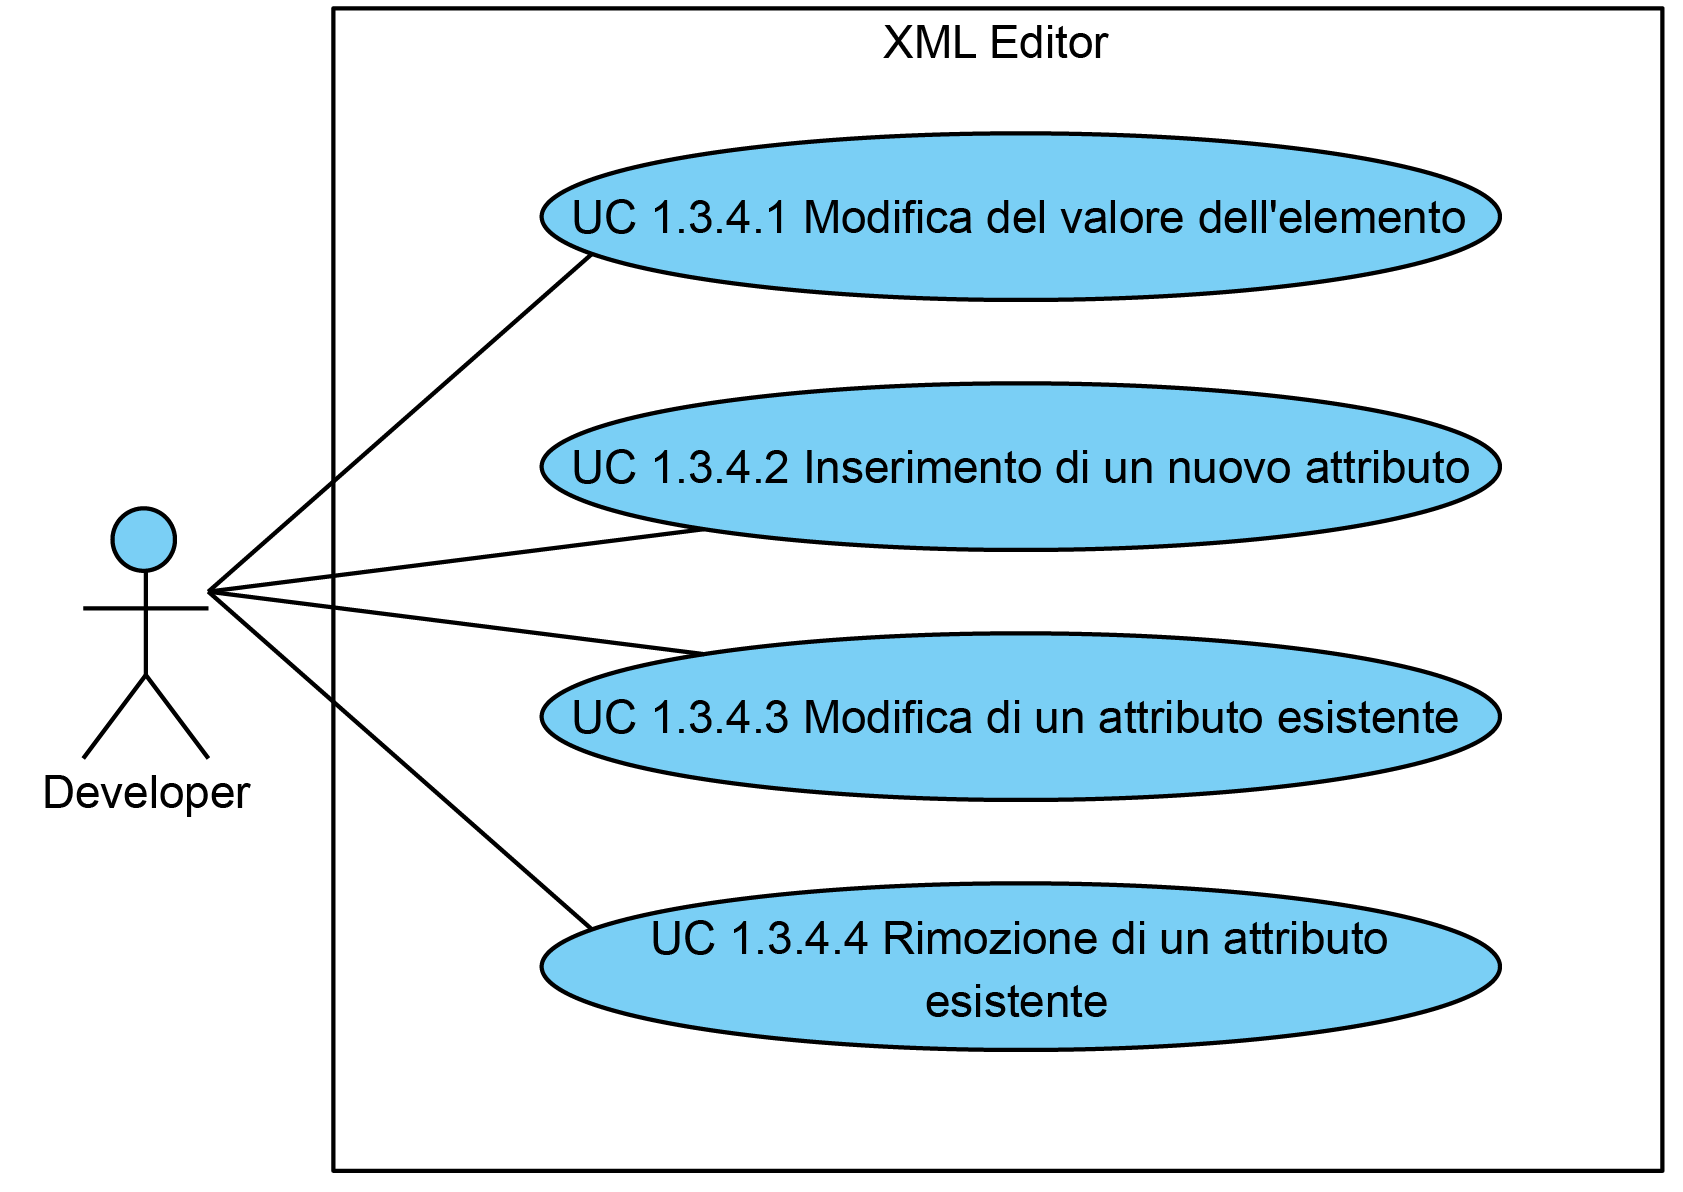
\includegraphics[width=0.9\columnwidth]{tool2/UC1-3-4.png} 
			\caption{Use Case - UC 1.3.4 Editing del nodo selezionato}
		\end{figure}
		
		\begin{itemize}
			\item\textbf{Attori}: developer.
			\item\textbf{Descrizione}: un developer deve poter editare il file XML correntemente visualizzato.
			\item\textbf{Precondizione}: il developer abbia selezionato l'azione per modificare l'elemento correntemente selezionato.
			\item\textbf{Flusso principale degli eventi}: 
			\begin{enumerate}
				\item \textit{l'utente ha la possibilità di:} \textit{modifica del valore dell'elemento} (\hyperref[subsec:XEUC1.3.4.1]{UC 1.3.4.1});
				
				\item \textit{l'utente ha la possibilità di:} \textit{inserimento di un nuovo attributo} (\hyperref[subsec:XEUC1.3.4.2]{UC 1.3.4.2});
				
				\item \textit{l'utente ha la possibilità di:} \textit{modifica di un attributo esistente} (\hyperref[subsec:XEUC1.3.4.3]{UC 1.3.4.3});
				
				\item \textit{l'utente ha la possibilità di:} \textit{rimozione di un attributo esistente} (\hyperref[subsec:XEUC1.3.4.4]{UC 1.3.4}).
				
			\end{enumerate}
			\item\textbf{Postcondizione}: il sistema ha modificato la versione caricata in memoria del file XML modificato.
		\end{itemize}
		
	\subsection{UC 1.3.4.1 Modifica del valore dell'elemento}
		\label{subsec:XEUC1.3.4.1}
		
		\begin{itemize}
			\item\textbf{Attori}: developer.
			\item\textbf{Descrizione}: il developer può modificare il valore dell'elemento.
			\item\textbf{Precondizione}: il developer abbia selezionato l'azione aggiungere per modificare un elemento.
			\item\textbf{Scenario principale}: il developer inserisce il nuovo value.
			\item\textbf{Postcondizione}: il sistema ha modificato il valore dell'elemento.
		\end{itemize}
		
	\subsection{UC 1.3.4.2 Inserimento di un nuovo attributo}
		\label{subsec:XEUC1.3.4.2}
		
		\begin{itemize}
			\item\textbf{Attori}: developer.
			\item\textbf{Descrizione}: il developer può aggiungere un attributo all'elemento.
			\item\textbf{Precondizione}: il developer abbia selezionato l'azione aggiungere per modificare un elemento.
			\item\textbf{Scenario principale}: il developer inserisce il nome del nuovo attributo ed il corrispettivo valore.
			\item\textbf{Postcondizione}: il sistema ha aggiunto un nuovo attributo con il nome ed il valore inseriti dal developer.
		\end{itemize}
		
	\subsection{UC 1.3.4.3 Modifica di un attributo esistente}
		\label{subsec:XEUC1.3.4.3}
		
		\begin{itemize}
			\item\textbf{Attori}: developer.
			\item\textbf{Descrizione}: il developer può modificare il valore e/o il nome di un attributo precedentemente inserito.
			\item\textbf{Precondizione}: il developer abbia selezionato l'azione aggiungere per modificare un elemento.
			\item\textbf{Scenario principale}: il developer inserisce il nome e/o il valore dell'attributo da modificare.
			\item\textbf{Postcondizione}: il sistema ha modificato l'attributo selezionato con i dati inseriti dal developer.
		\end{itemize}
		
	\subsection{UC 1.3.4.4 Rimozione di un attributo esistente}
		\label{subsec:XEUC1.3.4.4}
		
		\begin{itemize}
			\item\textbf{Attori}: developer.
			\item\textbf{Descrizione}: il developer può eliminare un attributo precedentemente inserito.
			\item\textbf{Precondizione}: il developer abbia selezionato l'azione aggiungere per modificare un elemento.
			\item\textbf{Scenario principale}: il developer seleziona l'attributo da eliminare.
			\item\textbf{Postcondizione}: il sistema ha eliminato l'attributo selezionato dal developer.
		\end{itemize}
		
	\subsection{UC 1.3.5 Duplicazione del nodo selezionato}
		\label{subsec:XEUC1.3.5}
		
		\begin{itemize}
			\item\textbf{Attori}: developer.
			\item\textbf{Descrizione}: viene aggiunta al padre del nodo selezionato una copia profonda di questo.
			\item\textbf{Precondizione}: il developer abbia selezionato l'azione di duplicazione di un nodo.
			\item\textbf{Scenario principale}: il developer seleziona il nodo da duplicare.
			\item\textbf{Postcondizione}: il sistema ha aggiunto al padre del nodo selezionato una copia profonda di tale nodo. Inoltre ha espanso l'albero fino al nuovo nodo creato.
		\end{itemize}
		
	\subsection{UC 1.3.6 Copia del nodo selezionato}
		\label{subsec:XEUC1.3.6}
		
		\begin{itemize}
			\item\textbf{Attori}: developer.
			\item\textbf{Descrizione}: viene fatta una copia profonda del nodo selezionato e conservata in memoria, pronta per essere incollata.
			\item\textbf{Precondizione}: il developer abbia selezionato l'azione di copia di un nodo.
			\item\textbf{Scenario principale}: il developer seleziona il nodo che intende copia.
			\item\textbf{Postcondizione}: il sistema ha memorizzato in memoria una copia profonda del nodo selezionato.
		\end{itemize}
		
	\subsection{UC 1.3.7 Incollare il nodo precedentemente copiato}
		\label{subsec:XEUC1.3.7}
		
		\begin{itemize}
			\item\textbf{Attori}: developer.
			\item\textbf{Descrizione}: viene aggiunto come figlio del nodo correttamente selezionato il nodo precedentemente copiato.
			\item\textbf{Precondizione}: il developer richiede di copiare il nodo precedentemente copiato.
			\item\textbf{Scenario principale}: il developer seleziona il nodo destinazione che conterrà il nuovo nodo.
			\item\textbf{Postcondizione}: il sistema ha aggiunto come figlio del nodo destinazione il nodo precedentemente copiato. Inoltre ha selezionato ed espanso l'albero fino al nuovo nodo aggiunto.
		\end{itemize}
		
	\subsection{UC 1.3.8 Rimozione del nodo selezionato}
		\label{subsec:XEUC1.3.8}
		
		\begin{itemize}
			\item\textbf{Attori}: developer.
			\item\textbf{Descrizione}: viene rimosso il nodo correntemente selezionato.
			\item\textbf{Precondizione}: il developer abbia selezionato l'azione di rimozione di un nodo.
			\item\textbf{Scenario principale}: il developer abbia selezionato il nodo da rimuovere.
			\item\textbf{Postcondizione}: il sistema ha rimosso il nodo selezionato.
		\end{itemize}
		
	\subsection{UC 1.3.9 Rimozione di tutti i nodi figli del nodo selezionato}
		\label{subsec:XEUC1.3.9}
		
		\begin{itemize}
			\item\textbf{Attori}: developer.
			\item\textbf{Descrizione}: vengono rimossi tutti i nodi figli del nodo correntemente selezionato.
			\item\textbf{Precondizione}: il developer abbia selezionato l'azione per rimuovere tutti i nodi figli.
			\item\textbf{Scenario principale}: il developer seleziona il nodo di cui si vuole rimuovere tutti i figli.
			\item\textbf{Postcondizione}: il sistema ha rimosso tutti i nodi del nodo attualmente selezionato.
		\end{itemize}
		
	\subsection{UC 1.3.10 Istanziazione di una nuova relazione}
		\label{subsec:XEUC1.3.10}
		
		\begin{itemize}
			\item\textbf{Attori}: developer.
			\item\textbf{Descrizione}: vengono creati in automatico tutti i nodi necessari per creare una relazione tra i nodi partenza selezionati e il nodo destinatario scelto.
			\item\textbf{Precondizione}: il developer abbia selezionato l'azione per creare in automatico una relazione.
			\item\textbf{Scenario principale}: il developer seleziona uno o più nodi e successivamente sceglie il nodo che riferirà i nodi precedentemente selezionati.
			\item\textbf{Postcondizione}: il sistema ha creato tutti i nodi necessari ad esplicitare le relazioni richieste.
		\end{itemize}
		
	\subsection{UC 1.3.11 Visualizzazione degli errori occorsi durante l'istanziazione di una nuova relazione}
		\label{subsec:XEUC1.3.11}
		
		\begin{itemize}
			\item\textbf{Attori}: developer.
			\item\textbf{Descrizione}: si è verificato uno dei seguenti errori durante l'istanziazione di una relazione:
			\begin{itemize}
				\item non esiste nessuna relazione per cui il nodo selezionato è riconoscibile come nodo partenza di una relazione;
				\item sono stati selezionati come nodi destinazione nodi non riconoscibili come destinazione di una relazione.
				\item non esiste nessun percorso di relazioni che lega il nodo partenza con il nodo destinazione selezionati;
				\item sono stati selezionati come nodi destinazione nodi di tipi differenti.
			\end{itemize}.
			\item\textbf{Precondizione}: il developer ha selezionato l'azione per creare una nuova relazione e specificato gli elementi da coinvolgere.
			\item\textbf{Scenario principale}: viene fornita una spiegazione dell'errore commesso e come risolverlo.
			\item\textbf{Postcondizione}: l'errore commesso è stato visualizzato e spiegato, non viene eseguita nessuna modifica al file XML.
		\end{itemize}
		
	\subsection{UC 1.3.12 Annullamento dell'ultima modifica eseguita}
		\label{subsec:XEUC1.3.12}
		
		\begin{itemize}
			\item\textbf{Attori}: developer.
			\item\textbf{Descrizione}: viene annullata l'ultima modifica e ripristinato lo stato precedente del file.
			\item\textbf{Precondizione}: il developer abbia selezionato l'azione per annullare l'ultima modifica ed è stata effettuata almeno una modifica al file XML.
			\item\textbf{Scenario principale}: viene ripristinato lo stato del file precedente alla modifica.
			\item\textbf{Postcondizione}: il sistema ha ripristinato lo stato del file prima dell'ultima azione di modifica.
		\end{itemize}
		
	\subsection{UC 1.3.13 Ripristino dell'ultima modifica annullata}
		\label{subsec:XEUC1.3.13}
		
		\begin{itemize}
			\item\textbf{Attori}: developer.
			\item\textbf{Descrizione}: viene ripristinata l'ultima modifica annullata.
			\item\textbf{Precondizione}: il developer abbia selezionato l'azione per ripristinare l'ultima modifica annullata ed è stata annullata almeno una modifica al file XML.
			\item\textbf{Scenario principale}: viene ripristinata l'ultima modifica annullata.
			\item\textbf{Postcondizione}: il sistema ha ripristinato lo stato del file prima dell'ultima azione di annullamento eseguita.
		\end{itemize}
		
	\subsection{UC 1.4 Salvare le modifiche di un file modificato}
		\label{subsec:XEUC1.4}
			
		\begin{itemize}
			\item\textbf{Attori}: developer.
			\item\textbf{Descrizione}: un developer deve poter salvare le modifiche effettuate su un file XML precedentemente aperto.
			\item\textbf{Precondizione}: il developer abbia selezionato l'azione per salvare un file XML e abbia almeno un file aperto e modificato.
			\item\textbf{Scenario principale}: viene salvato il file XML modificato.
			\item\textbf{Postcondizione}: il sistema ha salvato su disco le modifiche apportate al file XML.
		\end{itemize}
		
	\subsection{UC 1.5 Editing del filtro sul nome dell'attributo da visualizzare}
		\label{subsec:XEUC1.5}
		
		\begin{itemize}
			\item\textbf{Attori}: developer.
			\item\textbf{Descrizione}: un developer deve poter modificare il filtro che seleziona l'attributo cui valore è mostrato nell'albero rappresentante il file XML.
			\item\textbf{Precondizione}: il developer abbia lanciato il tool sotto un sistema Windows 7 o superiore.
			\item\textbf{Scenario principale}: il developer inserisce il nuovo filtro.
			\item\textbf{Postcondizione}: il sistema ha salvato il nuovo filtro e ha aggiornato la visualizzazione di tutti i file aperti.
		\end{itemize}
		
	\subsection{UC 1.6 Editing dei file associati}
		\label{subsec:XEUC1.6}
		
		\begin{figure}[!h] 
			\centering 
			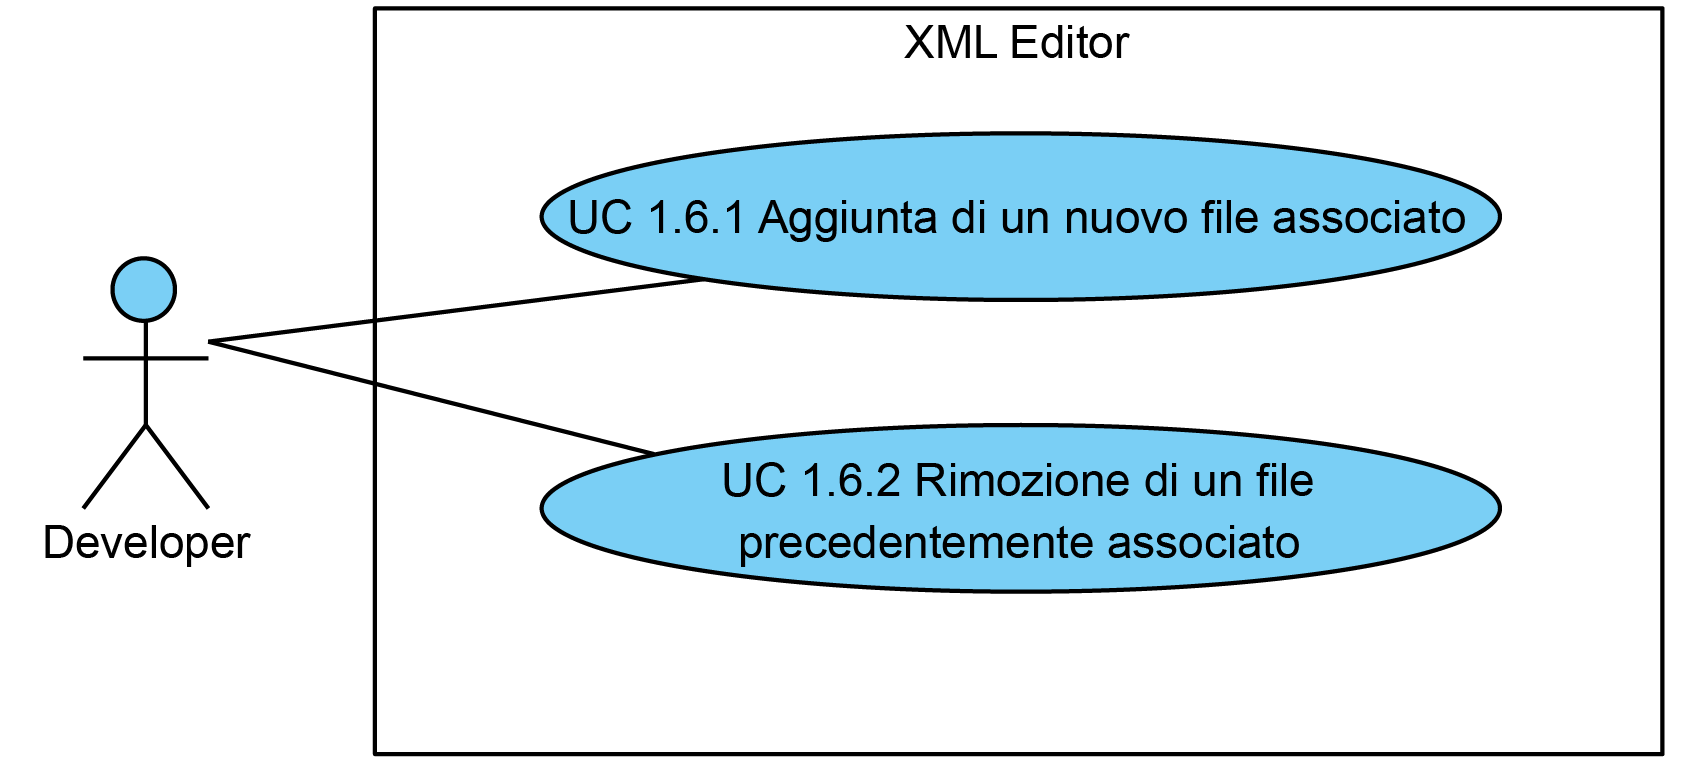
\includegraphics[width=0.9\columnwidth]{tool2/UC1-6.png} 
			\caption{Use Case - UC 1.6 Editing dei file associati}
		\end{figure}
		
		\begin{itemize}
			\item\textbf{Attori}: developer.
			\item\textbf{Descrizione}: un developer deve poter aggiungere e rimuovere i file associati.
			\item\textbf{Precondizione}: il developer ha caricato correttamente un file XML.
			\item\textbf{Flusso principale degli eventi}: 
			\begin{enumerate}
				\item \textit{l'utente ha la possibilità di:} \textit{aggiunta di un nuovo file associato} (\hyperref[subsec:XEUC1.6.1]{UC 1.6.1});
				
				\item \textit{l'utente ha la possibilità di:} \textit{rimozione di un file precedentemente associato} (\hyperref[subsec:XEUC1.6.2]{UC1.6.2}).
				
			\end{enumerate}
			\item\textbf{Postcondizione}: il sistema ha modificato i file associati del file XML principale attualmente aperto.
		\end{itemize}
		
	\subsection{UC 1.6.1 Aggiunta di un nuovo file associato}
		\label{subsec:XEUC1.6.1}
		
		\begin{itemize}
			\item\textbf{Attori}: developer.
			\item\textbf{Descrizione}: un developer deve poter aggiungere un nuovo file associato al corrente file principale.
			\item\textbf{Precondizione}: il developer abbia selezionato l'azione di modifica dei file associati.
			\item\textbf{Scenario principale}: il developer inserisce il percorso ed il nome del nuovo file associato.
			\item\textbf{Postcondizione}: il sistema ha salvato il nuovo file associato lo carica.
		\end{itemize}
		
	\subsection{UC 1.6.2 Rimozione di un file precedentemente associato}
		\label{subsec:XEUC1.6.2}
		
		\begin{itemize}
			\item\textbf{Attori}: developer.
			\item\textbf{Descrizione}: un developer deve poter rimuovere un file associato dal corrente file principale.
			\item\textbf{Precondizione}: il developer abbia selezionato l'azione di modifica dei file associati.
			\item\textbf{Scenario principale}: il developer seleziona il file da rimuovere.
			\item\textbf{Postcondizione}: il sistema ha rimosso il file selezionato. La copia in memoria del file non è stata eliminata.
		\end{itemize}
		
	\subsection{UC 1.7 Editing delle relazioni}
		\label{subsec:XEUC1.7}
		
		\begin{figure}[!h] 
			\centering 
			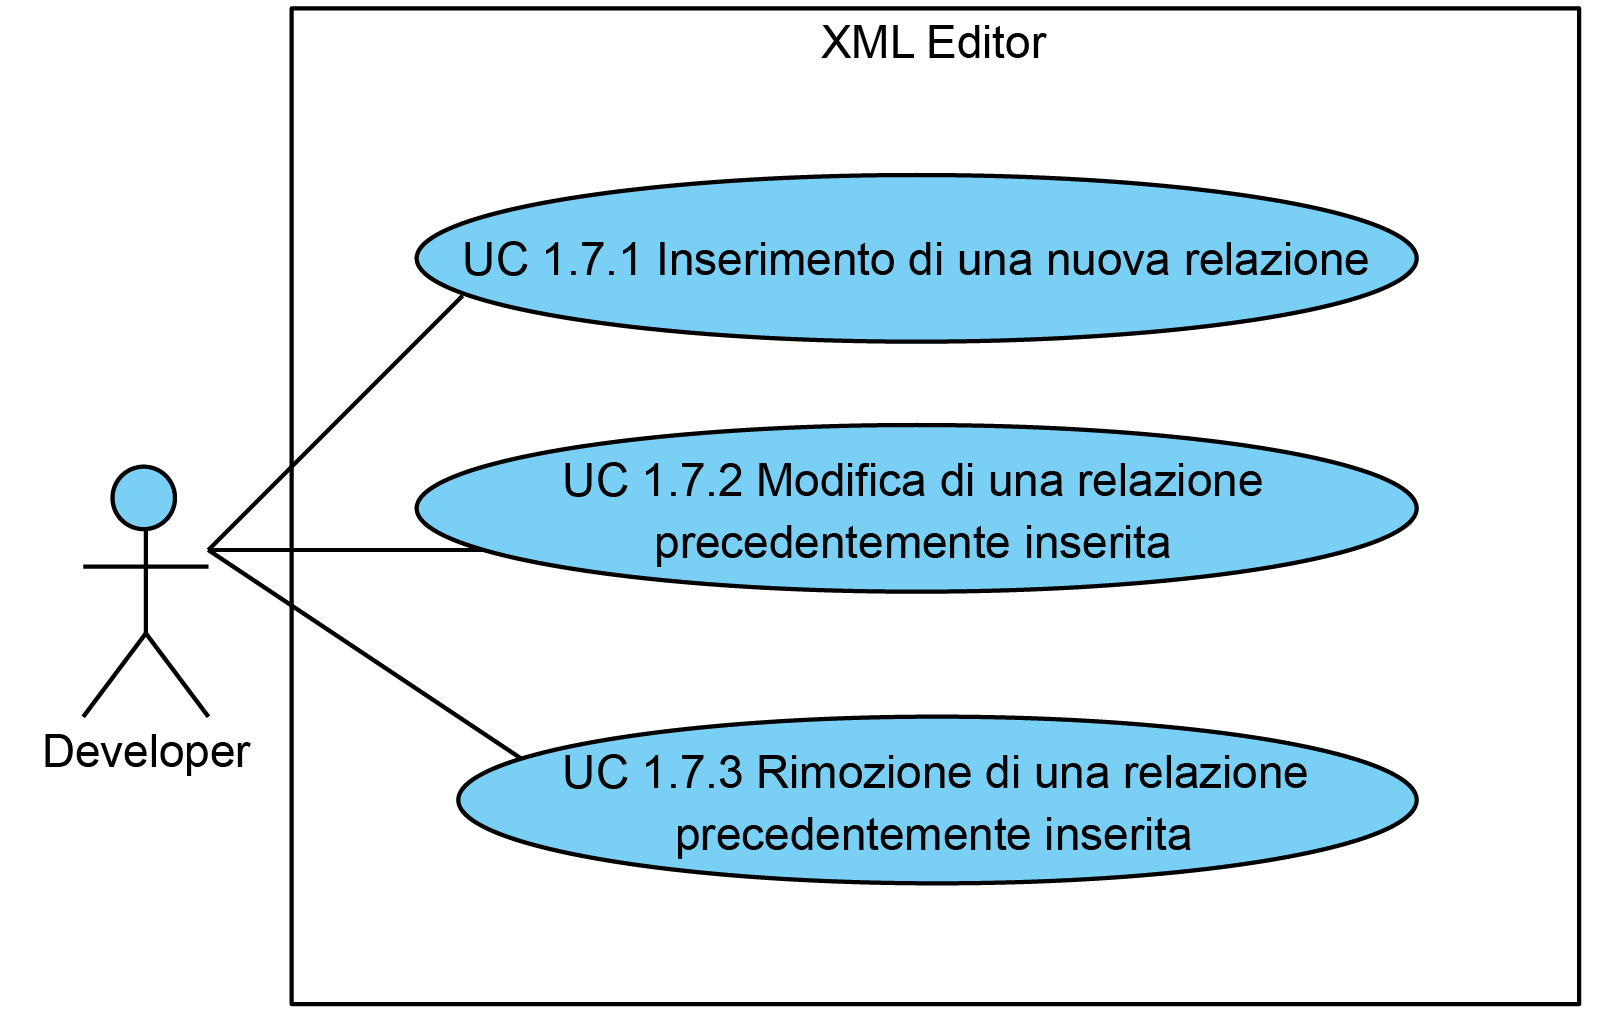
\includegraphics[width=0.9\columnwidth]{tool2/UC1-7.png} 
			\caption{Use Case - UC 1.7 Editing delle relazioni}
		\end{figure}
		
		\begin{itemize}
			\item\textbf{Attori}: developer.
			\item\textbf{Descrizione}: un developer deve poter editare le relazioni presenti.
			\item\textbf{Precondizione}: il developer ha lanciato il tool sotto un sistema Windows 7 o superiore.
			\item\textbf{Flusso principale degli eventi}: 
			\begin{enumerate}
				\item \textit{l'utente ha la possibilità di:} \textit{inserimento di una nuova relazione} (\hyperref[subsec:XEUC1.7.1]{UC 1.7.1});
				
				\item \textit{l'utente ha la possibilità di:} \textit{modifica di una relazione precedentemente inserita} (\hyperref[subsec:XEUC1.7.2]{UC1.7.2});
				
				\item \textit{l'utente ha la possibilità di:} \textit{rimozione di una relazione precedentemente inserita} (\hyperref[subsec:XEUC1.7.3]{UC1.7.3}).
				
			\end{enumerate}
			\item\textbf{Postcondizione}: il sistema ha modificato le relazione come desiderato dall'utente.
		\end{itemize}
		
	\subsection{UC 1.7.1 Inserimento di una nuova relazione}
		\label{subsec:XEUC1.7.1}
		
		\begin{itemize}
			\item\textbf{Attori}: developer.
			\item\textbf{Descrizione}: un developer deve poter aggiungere una nuova relazione.
			\item\textbf{Precondizione}: il developer abbia selezionato l'azione di modifica delle relazioni.
			\item\textbf{Scenario principale}: il developer inserisce tutte le informazioni necessarie alla creazione di una relazione.
			\item\textbf{Postcondizione}: il sistema ha memorizzato la nuova relazione.
		\end{itemize}
		
	\subsection{UC 1.7.2 Modifica di una relazione precedentemente inserita}
		\label{subsec:XEUC1.7.2}
		
		\begin{itemize}
			\item\textbf{Attori}: developer.
			\item\textbf{Descrizione}: un developer deve poter modificare una relazione precedentemente inserita.
			\item\textbf{Precondizione}: il developer abbia selezionato l'azione di modifica delle relazioni e la relazione da modificare.
			\item\textbf{Scenario principale}: il developer inserisce tutte le informazioni che vuole modificare della relazione.
			\item\textbf{Postcondizione}: il sistema ha memorizzato i cambiamenti nella relazione selezionata.
		\end{itemize}
		
	\subsection{UC 1.7.3 Rimozione di una relazione precedentemente inserita}
		\label{subsec:XEUC1.7.3}
		
		\begin{itemize}
			\item\textbf{Attori}: developer.
			\item\textbf{Descrizione}: un developer deve poter rimuovere una relazione.
			\item\textbf{Precondizione}: il developer abbia selezionato l'azione di modifica delle relazioni.
			\item\textbf{Scenario principale}: il developer seleziona la relazione da rimuovere.
			\item\textbf{Postcondizione}: il sistema ha rimosso la relazione selezionata.
		\end{itemize}
		
	\subsection{UC 1.8 Importazione delle relazioni da file}
		\label{subsec:XEUC1.8}
		
		\begin{itemize}
			\item\textbf{Attori}: developer.
			\item\textbf{Descrizione}: un developer deve poter importare e sostituire le relazioni correnti con le relazione contenute in un file di configurazione precedentemente esportato.
			\item\textbf{Precondizione}: il developer ha selezionato l'azione per importare le relazioni da un file.
			\item\textbf{Scenario principale}: il developer inserisce il percorso ed il nome del file contenente le relazioni.
			\item\textbf{Postcondizione}: il sistema ha rimosso tutte le precedenti relazioni e le ha sostituite con tutte quelle presenti nel file.
		\end{itemize}
		
	\subsection{UC 1.9 Esportazione delle relazioni su file}
		\label{subsec:XEUC1.9}
		
		\begin{itemize}
			\item\textbf{Attori}: developer.
			\item\textbf{Descrizione}: un developer deve poter esportare le relazioni attualmente inserite su file.
			\item\textbf{Precondizione}: il developer ha selezionato l'azione per esportare le relazioni su file.
			\item\textbf{Scenario principale}: il developer inserisce il percorso ed il nome del file dove esportare le relazioni.
			\item\textbf{Postcondizione}: il sistema esportato le relazioni nel file selezionato.
		\end{itemize}
		
	\subsection{UC 1.10 Avvio del check sulle relazioni}
		\label{subsec:XEUC1.10}
		
		\begin{itemize}
			\item\textbf{Attori}: developer.
			\item\textbf{Descrizione}: un developer deve poter verificare la consistenza delle relazioni presenti nel file principale e in tutti i file associati sulla base delle relazioni inserite.
			\item\textbf{Precondizione}: il developer ha selezionato l'azione per verificare la consistenza delle relazioni. Almeno un file XML deve essere stato aperto con successo.
			\item\textbf{Scenario principale}: il developer seleziona l'azione per effettuare il check delle relazioni.
			\item\textbf{Postcondizione}: il sistema ha verificato le relazioni nel file principale e in tutti gli associati.
		\end{itemize}
		
	\subsection{UC 1.11 Visualizzazione del risultato del check sulle relazioni}
		\label{subsec:XEUC1.11}
		
		\begin{figure}[!h] 
			\centering 
			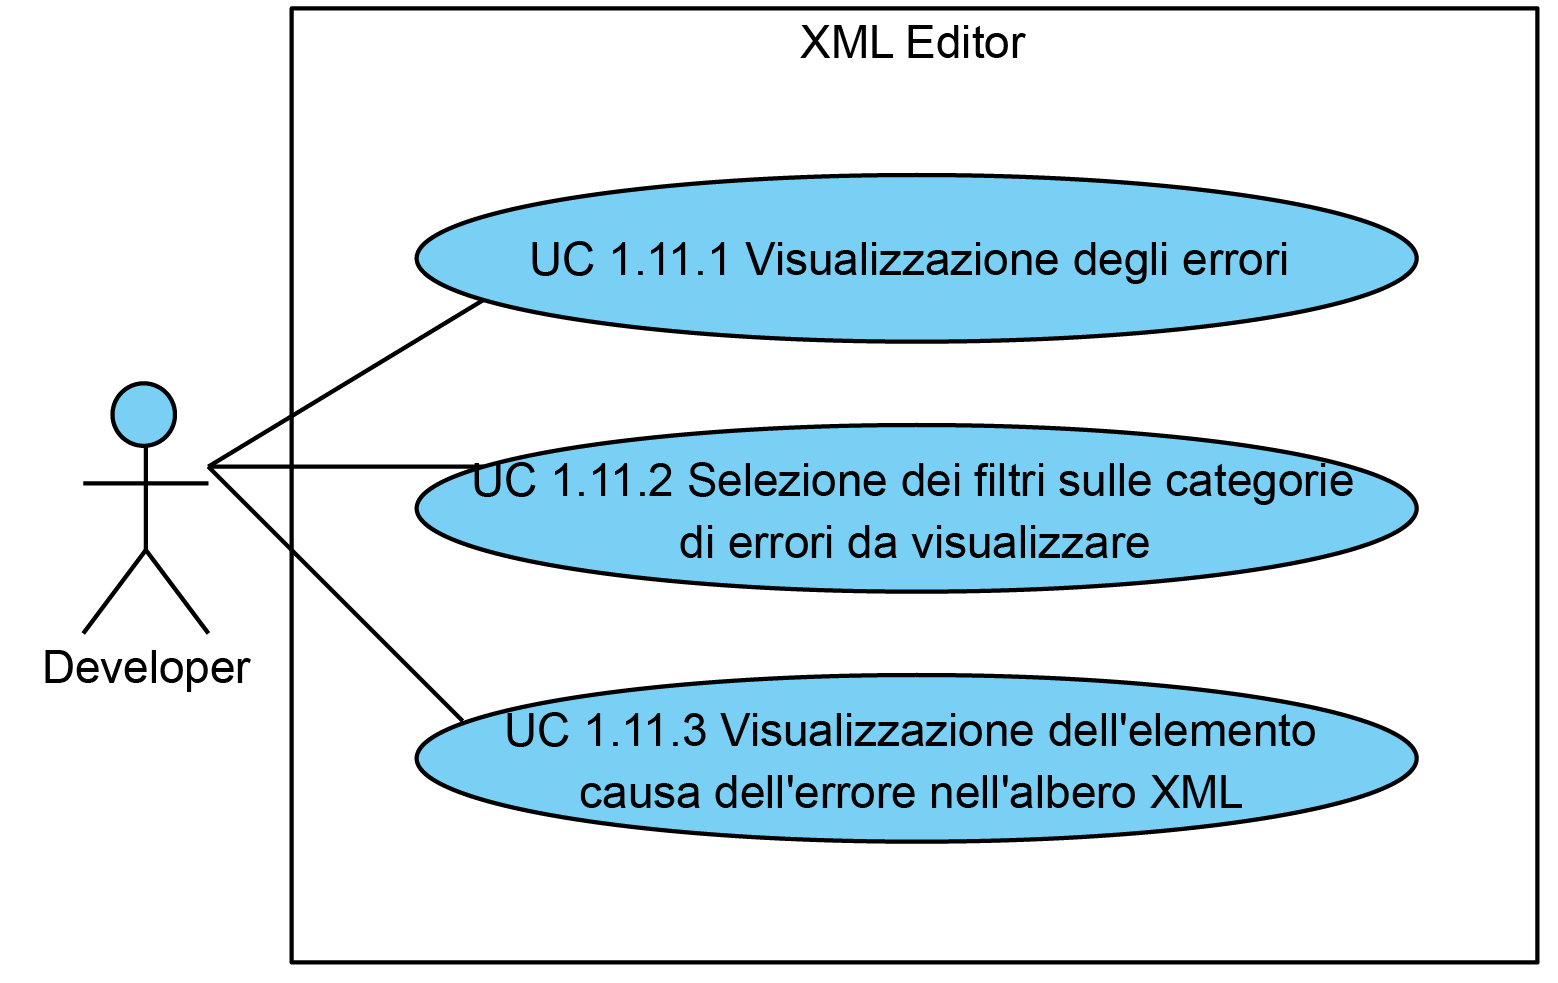
\includegraphics[width=0.9\columnwidth]{tool2/UC1-11.png} 
			\caption{Use Case - UC 1.11 Visualizzazione del risultato del check sulle relazioni}
		\end{figure}
		
		\begin{itemize}
			\item\textbf{Attori}: developer.
			\item\textbf{Descrizione}: un developer deve visualizzare l'esito del check sulle relazioni.
			\item\textbf{Precondizione}: il developer ha avviato il check sulle relazioni e quest'ultimo è terminato.
			\item\textbf{Flusso principale degli eventi}: 
			\begin{enumerate}
				\item \textit{l'utente ha la possibilità di:} \textit{visualizzazione degli errori} (\hyperref[subsec:XEUC1.11.1]{UC 1.11.1});
				
				\item \textit{l'utente ha la possibilità di:} \textit{selezione dei filtri sulle categorie di errori da visualizzare} (\hyperref[subsec:XEUC1.11.2]{UC1.11.2});
				
				\item \textit{l'utente ha la possibilità di:} \textit{visualizzazione dell'elemento causa dell'errore nell'albero XML} (\hyperref[subsec:XEUC1.11.3]{UC1.11.3}).
				
			\end{enumerate}
			\item\textbf{Postcondizione}: il sistema ha permesso la visualizzazione dei risultati del check sulle relazioni.
		\end{itemize}
		
	\subsection{UC 1.11.1 Visualizzazione degli errori}
		\label{subsec:XEUC1.11.1}
		
		\begin{itemize}
			\item\textbf{Attori}: developer.
			\item\textbf{Descrizione}: un developer deve poter l'esito della verifica delle relazioni.
			\item\textbf{Precondizione}: il developer ha avviato il check sulle relazioni e quest'ultimo è terminato.
			\item\textbf{Scenario principale}: viene visualizzato per ogni errore: la severità, la tipologia, la descrizione, il nome del file in cui l'errore è stato trovato.
			\item\textbf{Postcondizione}: il sistema ha visualizzato l'output della verifica delle relazioni.
		\end{itemize}
		
	\subsection{UC 1.11.2 Selezione dei filtri sulle categorie di errori da visualizzare}
		\label{subsec:XEUC1.11.2}
		
		\begin{itemize}
			\item\textbf{Attori}: developer.
			\item\textbf{Descrizione}: un developer deve poter selezionare i filtri sulla severità degli errori.
			\item\textbf{Precondizione}: il developer ha avviato il check sulle relazioni e quest'ultimo è terminato.
			\item\textbf{Scenario principale}: il developer seleziona per ogni categoria di severità se desidera visualizzare gli errori di quella categoria.
			\item\textbf{Postcondizione}: la visualizzazione viene aggiornata e vengono mostrati solo gli errori per il quale corrispettivo filtro di severità è attivo.
		\end{itemize}
		
	\subsection{UC 1.11.3 Visualizzazione dell'elemento causa dell'errore nell'albero XML}
		\label{subsec:XEUC1.11.3}
		
		\begin{itemize}
			\item\textbf{Attori}: developer.
			\item\textbf{Descrizione}: un developer deve poter visualizzare l'elemento causa dell'errore nel suo albero XML di appartenenza.
			\item\textbf{Precondizione}: il developer ha avviato il check sulle relazioni seleziona l'azione per mostrare l'elemento causa dell'errore.
			\item\textbf{Scenario principale}: il developer seleziona l'azione per visualizzare il nodo causa dell'errore nel suo albero di appartenenza.
			\item\textbf{Postcondizione}: il sistema ha visualizzato il nodo nel contesto del suo albero di appartenenza.
		\end{itemize}
		
	\subsection{UC 1.12 Visualizzazione dell'about del programma}
		\label{subsec:XEUC1.12}
		
		\begin{itemize}
			\item\textbf{Attori}: developer.
			\item\textbf{Descrizione}: un developer deve poter visualizzare la finestra about del programma.
			\item\textbf{Precondizione}: il developer abbia selezionato l'azione per visualizzare la finestra about del programma.
			\item\textbf{Scenario principale}: il developer visualizza l'about sul programma.
			\item\textbf{Postcondizione}: il sistema ha mostrato la finestra about del programma.
		\end{itemize}
		
	\subsection{UC 1.13 Visualizzazione degli errori occorsi durante l'apertura del file}
		\label{subsec:XEUC1.13}
		
		\begin{itemize}
			\item\textbf{Descrizione}: si è verificato uno dei seguenti errori durante l'apertura di un file XML:
			\begin{itemize}
				\item il percorso inserito non è valido;
				\item il file indicato non esiste;
				\item il file indicato non è leggibile;
				\item si è verificato un errore non gestito durante l'apertura del file;
				\item il parser XML ha trovato un errore sintattico nel file XML.
			\end{itemize}
			\item\textbf{Precondizione}: il developer ha selezionato l'azione per aprire un file esistente e abbia inserito il percorso ed il nome del file.
			\item\textbf{Scenario principale}: viene fornita una spiegazione dell'errore commesso e come risolverlo.
			\item\textbf{Postcondizione}: l'errore commesso è stato visualizzato e spiegato, il file XML non è stato aperto. Il precedente lavoro è stato chiuso.
		\end{itemize}
		
	\subsection{UC 1.14 Visualizzazione degli errori occorsi durante il salvataggio del file}
		\label{subsec:XEUC1.14}
		
		\begin{itemize}
			\item\textbf{Descrizione}: si è verificato uno dei seguenti errori durante il salvataggio su disco di un file XML:
			\begin{itemize}
				\item il file indicato non è scrivibile;
				\item si è verificato un errore non gestito durante l'apertura in scrittura del file.
			\end{itemize}
			\item\textbf{Precondizione}: il developer ha selezionato l'azione per il salvataggio del file modificato.
			\item\textbf{Scenario principale}: viene fornita una spiegazione dell'errore commesso e come risolverlo.
			\item\textbf{Postcondizione}: l'errore commesso è stato visualizzato e spiegato, il file XML non è stato salvato. Il precedente lavoro non è stato perso.
		\end{itemize}
		
	\subsection{UC 1.15 Visualizzazione degli errori occorsi durante l'importazione}
		\label{subsec:XEUC1.15}
		
		\begin{itemize}
			\item\textbf{Descrizione}: si è verificato uno dei seguenti errori durante l'importazione delle relazioni:
			\begin{itemize}
				\item il percorso inserito non è valido;
				\item il file indicato non esiste;
				\item il file indicato non è leggibile;
				\item si è verificato un errore non gestito durante l'apertura del file;
				\item il parser XML ha trovato un errore sintattico nel file.
			\end{itemize}
			\item\textbf{Precondizione}: il developer ha selezionato l'azione per l'importazione delle relazioni da filee ha inserito un percorso ed il nome del file.
			\item\textbf{Scenario principale}: viene fornita una spiegazione dell'errore commesso e come risolverlo.
			\item\textbf{Postcondizione}: l'errore commesso è stato visualizzato e spiegato, le relazioni non sono state importate. Le precedenti relazioni non sono state eliminate.
		\end{itemize}
		
	\subsection{UC 1.16 Visualizzazione degli errori occorsi durante l'esportazione}
		\label{subsec:XEUC1.16}
		
		\begin{itemize}
			\item\textbf{Descrizione}: si è verificato uno dei seguenti errori durante l'esportazione delle relazioni su un nuovo file:
			\begin{itemize}
				\item il file indicato non è scrivibile;
				\item si è verificato un errore non gestito durante l'apertura in scrittura del file.
			\end{itemize}
			\item\textbf{Precondizione}: il developer ha selezionato l'azione per l'esportazione delle relazioni su file.
			\item\textbf{Scenario principale}: viene fornita una spiegazione dell'errore commesso e come risolverlo.
			\item\textbf{Postcondizione}: l'errore commesso è stato visualizzato e spiegato, le relazioni non sono state esportate.
		\end{itemize}


\section{Tracciamento dei requisiti}
	Partendo dai casi d'uso si è provveduto a stilare una precisa analisi dei requisiti per il tool in questione. I requisiti trovati sono stati inoltre tracciati in relazione al caso d'uso di origine.\\
	
	Di seguito vengono riportati tutti i requisiti individuati. Per essere più leggibili verranno separati in tabelle a seconda della loro categoria. Di ogni requisito verranno indicati: tipologia, importanza e provenienza.\\
	I requisiti dovranno essere classificati per tipo e importanza e utilizzeranno la seguente sintassi:
	\begin{center}
		R[Importanza][Tipo][Codice]
	\end{center}
	\begin{itemize}
		\item \textbf{Importanza}: può assumere solo uno fra i seguenti valori:
		\begin{itemize}
			\item \textit{0}: requisito obbligatorio;
			\item \textit{1}: requisito desiderabile;
			\item \textit{2}: requisito opzionale.
		\end{itemize}
		\item \textbf{Tipo}: pu\`{o} assumere solo uno fra i seguenti valori:
		\begin{itemize}
			\item  \textit{F}: funzionale;
			\item  \textit{Q}: di qualità;
			\item  \textit{P}: prestazionale;
			\item  \textit{V}: vincolo.
		\end{itemize}
		\item \textbf{Codice}: è il codice gerarchico univoco di ogni vincolo espresso in numeri (esempio: 1.3.2).
	\end{itemize}

	Per ogni requisito vengono inoltre specificati:
	\begin{itemize}
		\item \textbf{descrizione}: breve ma completa ed il \underline{meno} ambigua possibile;
		\item \textbf{fonte}: pu\`{o} essere soltanto una o pi\`{u} tra le seguenti:
		\begin{itemize}
			\item \textit{caso d'uso}: il requisito \`{e} stato estrapolato da un caso d'uso. In questo caso va indicato il codice univoco del caso d'uso. \`{E} possibile indicare come fonte pi\`{u} di un caso d'uso.
			\item \textit{interno}: è stato ritenuto giusto aggiungere questo requisito per completezza.
			\item \textit{tutor aziendale}: il requisito è stato espressamente richiesto dal tutor aziendale.
		\end{itemize}
	\end{itemize}

\subsection{Requisiti funzionali}
\begin{center}
	\begin{longtable}{p{4.2cm}!{\color{white}\vrule width 0.5mm}p{6cm}!{\color{white}\vrule width 0.5mm}p{2.5cm}!{\color{white}\vrule width 0.5mm}}
		\rowcolor{headcolor}\textcolor{white}{\textbf{Requisito}}&\textcolor{white}{\textbf{Descrizione}}&\textcolor{white}{\textbf{Fonti}}\\
		
		\rowcolor{row1}\hspace{0mm}\hypertarget{XER0F1}{R0F1} & Un utente può creare un nuovo file XML. & \hyperref[subsec:XEUC1.1]{UC 1.1}\\
		
			\rowcolor{row2}\hspace{2mm}\hypertarget{XER0F1.1}{R0F1.1} & La creazione di un nuovo file XML richiede l'inserimento del percorso dove memorizzarlo. & \hyperref[subsec:XEUC1.1.1]{UC 1.1.1}\\
		
			\rowcolor{row1}\hspace{2mm}\hypertarget{XER0F1.2}{R0F1.2} & La creazione di un nuovo file XML richiede l'inserimento del nome del file. & \hyperref[subsec:XEUC1.1.2]{UC 1.1.2}\\
			
			
			\rowcolor{row2}\hspace{2mm}\hypertarget{XER0F1.3}{R0F1.3} & Se il file inserito è già presente nel sistema, il contenuto verrà sovrascritto solo nel momento del primo salvataggio. & Interno\\
			
		
		\rowcolor{row1}\hspace{0mm}\hypertarget{XER0F2}{R0F2} & Un utente può aprire un file XML preesistente. & \hyperref[subsec:XEUC1.2]{UC 1.2}\\
		
			\rowcolor{row2}\hspace{2mm}\hypertarget{XER0F2.1}{R0F2.1} & L'apertura di file XML richiede l'inserimento del percorso dove recuperarlo. & \hyperref[subsec:XEUC1.2]{UC 1.2}\\
		
			\rowcolor{row1}\hspace{2mm}\hypertarget{R0F2.2}{R0F2.2} & L'apertura di file XML richiede l'inserimento del nome del file da aprire. & \hyperref[subsec:XEUC1.2]{UC 1.2}\\
		
			\rowcolor{row2}\hspace{2mm}\hypertarget{R0F2.3}{R0F2.3} & Se prima dell'apertura di un file XML l'utente ha delle modifiche non salvate su qualche file, il sistema, per ogni file, chiede all'utente se cancellare l'azione, salvare o scartare le modifiche al lavoro precedente. & \hyperref[subsec:XEUC1.2]{UC 1.2}\\
		
	
		\rowcolor{row1}\hspace{0mm}\hypertarget{XER0F3}{R0F3} & Un utente può editare un file XML correntemente aperto e visualizzato. & \hyperref[subsec:XEUC1.3]{UC 1.3}\\
	
			\rowcolor{row2}\hspace{2mm}\hypertarget{XER0F3.1}{R0F3.1} & Un utente può selezionare e visualizzare l'elemento riferito da un elemento. & \hyperref[subsec:XEUC1.3.1]{UC 1.3.1}\\
	
				\rowcolor{row1}\hspace{4mm}\hypertarget{XER0F3.1.1}{R0F3.1.1} & Deve esistere una relazione nel database ed essere istanziata correttamente nell'XML. & Interno\\
	
			\rowcolor{row2}\hspace{2mm}\hypertarget{XER0F3.2}{R0F3.2} & Il programma mostra gli eventuali errori occorsi durante la ricerca del nodo destinazione della relazione. & \hyperref[subsec:XEUC1.3.2]{UC 1.3.2}\\
	
			\rowcolor{row1}\hspace{2mm}\hypertarget{XER0F3.2}{R0F3.2} & Il programma mostra gli eventuali errori occorsi durante la ricerca del nodo destinazione della relazione. & \hyperref[subsec:XEUC1.3.2]{UC 1.3.2}\\
	
			\rowcolor{row2}\hspace{2mm}\hypertarget{XER0F3.3}{R0F3.3} & Un utente può inserire un nuovo nodo figlio ad un elemento. & \hyperref[subsec:XEUC1.3.3]{UC 1.3.3}\\
			
				\rowcolor{row1}\hspace{4mm}\hypertarget{XER0F3.3.1}{R0F3.3.1} & Il programma apre automaticamente la schermata di editing del nuovo nodo inserito. & Tutor interno\\
	
			\rowcolor{row2}\hspace{2mm}\hypertarget{XER0F3.4}{R0F3.4} & Un utente può modificare un nodo dell'albero XML. & \hyperref[subsec:XEUC1.3.4]{UC 1.3.4}\\
			
				\rowcolor{row1}\hspace{4mm}\hypertarget{XER0F3.4.1}{R0F3.4.1} & Un utente può modificare il valore dell'elemento. & \hyperref[subsec:XEUC1.3.4.1]{UC 1.3.4.1}\\
	
				\rowcolor{row2}\hspace{4mm}\hypertarget{XER0F3.4.2}{R0F3.4.2} & Un utente può appendere un nuovo attributo all'elemento. & \hyperref[subsec:XEUC1.3.4.2]{UC 1.3.4.2}\\
	
				\rowcolor{row1}\hspace{4mm}\hypertarget{XER0F3.4.3}{R0F3.4.3} & Un utente può modificare un attributo esistente. & \hyperref[subsec:XEUC1.3.4.3]{UC 1.3.4.3}\\
	
				\rowcolor{row2}\hspace{4mm}\hypertarget{XER0F3.4.4}{R0F3.4.4} & Un utente può rimuovere un attributo esistente. & \hyperref[subsec:XEUC1.3.4.4]{UC 1.3.4.4}\\
	
				\rowcolor{row1}\hspace{4mm}\hypertarget{XER0F3.4.5}{R0F3.4.5} & Il programma blocca il salvataggio se l'utente ha inserito due attributi con lo stesso nome. & Interno\\
	
			\rowcolor{row2}\hspace{2mm}\hypertarget{XER0F3.5}{R0F3.5} & Un utente può duplicare un nodo, inserendo la copia come fratello del nodo copiato. & \hyperref[subsec:XEUC1.3.5]{UC 1.3.5}\\
	
			\rowcolor{row1}\hspace{2mm}\hypertarget{XER0F3.6}{R0F3.6} & Un utente può copiare un nodo e mantenerlo in memoria per essere incollato in un momento successivo. & \hyperref[subsec:XEUC1.3.6]{UC 1.3.6}\\
				
				\rowcolor{row2}\hspace{4mm}\hypertarget{XER0F3.6.1}{R0F3.6.1} & Il programma mantiene un solo nodo copiato alla volta. & Interno\\
	
				\rowcolor{row1}\hspace{4mm}\hypertarget{XER0F3.6.2}{R0F3.6.2} & Ogni nuovo nodo copiato sostituisce quelli precedenti. & Interno\\
	
				\rowcolor{row2}\hspace{4mm}\hypertarget{XER0F3.6.3}{R0F3.6.3} & Se il nodo origine della copia e viene modificato, la copia rimane immutata. & Interno\\
	
			\rowcolor{row1}\hspace{2mm}\hypertarget{XER0F3.7}{R0F3.7} & Un utente può incollare il nodo precedentemente copiato. & \hyperref[subsec:XEUC1.3.7]{UC 1.3.7}\\
	
			\rowcolor{row2}\hspace{2mm}\hypertarget{XER0F3.8}{R0F3.8} & Un utente può rimuovere un nodo. & \hyperref[subsec:XEUC1.3.8]{UC 1.3.8}\\
				
				\rowcolor{row1}\hspace{4mm}\hypertarget{XER0F3.8}{R0F3.8} & Quando il programma rimuove un nodo, vengono rimossi anche tutti i nodi discendenti. & Interno\\
	
			\rowcolor{row2}\hspace{2mm}\hypertarget{XER0F3.9}{R0F3.9} & Un utente può rimuovere tutti i discendenti di un nodo. & \hyperref[subsec:XEUC1.3.9]{UC 1.3.9}\\
			
			\rowcolor{row1}\hspace{2mm}\hypertarget{XER0F3.10}{R0F3.10} & Un utente può istanziare un nuova relazione in automatico, senza dover creare manualmente gli elementi necessari. & \hyperref[subsec:XEUC1.3.10]{UC 1.3.10}\\
			
				\rowcolor{row2}\hspace{4mm}\hypertarget{XER0F3.10.1}{R0F3.10.1} & Affinché l'operazione avvenga con successo è necessario che sia presente un percorso di relazioni che consente di effettuare l'operazione. & Interno\\
	
				\rowcolor{row1}\hspace{4mm}\hypertarget{XER0F3.10.2}{R0F3.10.2} & Se il percorso di relazioni contiene più di un elemento, allora il programma creerà dei nodi intermedi per completare l'operazione. & Interno\\
	
			\rowcolor{row2}\hspace{2mm}\hypertarget{XER0F3.11}{R0F3.11} & Il programma mostra gli eventuali errori occorsi durante l'istanziazione automatica di una relazione. & \hyperref[subsec:XEUC1.3.11]{UC 1.3.11}\\
	
	
			\rowcolor{row1}\hspace{2mm}\hypertarget{XER0F3.12}{R0F3.12} & Un utente può annullare l'ultima modifica effettuata. & \hyperref[subsec:XEUC1.3.12]{UC 1.3.12}\\
			
			\rowcolor{row2}\hspace{2mm}\hypertarget{XER0F3.13}{R0F3.13} & Un utente può ripristinare l'ultima modifica annullata. & \hyperref[subsec:XEUC1.3.13]{UC 1.3.13}\\
	
	
	
			\rowcolor{row1}\hspace{2mm}\hypertarget{R0F3.14}{R0F3.14} & Quando viene effettuata una modifica ad un file XML, viene aggiunto il carattere \sq{*} alla fine del nome per indicare all'utente il nuovo stato del file. & Interno\\
		
		
		\rowcolor{row2}\hspace{0mm}\hypertarget{XER0F4}{R0F4} & Un utente può salvare le modifiche effettuata ad un file XML. & \hyperref[subsec:XEUC1.4]{UC 1.4}\\
		
			\rowcolor{row1}\hspace{0mm}\hypertarget{XER0F4.1}{R0F4.1} & Il programma permette di salvare solo un file su cui sono state apportate modifiche. & \hyperref[subsec:XEUC1.4]{UC 1.4}\\
		
		\rowcolor{row2}\hspace{0mm}\hypertarget{XER0F5}{R0F5} & Un utente può modificare il filtro utilizzato per selezionare l'attributo il cui valore viene mostrato nell'albero per rappresentare l'elemento. & \hyperref[subsec:XEUC1.5]{UC 1.5}\\
			
			\rowcolor{row1}\hspace{0mm}\hypertarget{XER0F5.1}{R0F5.1} & Il valore inserito dall'utente viene memorizzato nel registro di sistema e ripristinato ad ogni apertura del programma. & \hyperref[subsec:XEUC1.5]{UC 1.5}\\
			
		\rowcolor{row2}\hspace{0mm}\hypertarget{XER0F6}{R0F6} & Un utente può modificare i file associati al file correntemente aperto. & \hyperref[subsec:XEUC1.6]{UC 1.6}\\
			
			\rowcolor{row1}\hspace{2mm}\hypertarget{XER0F6.1}{R0F6.1} & Un utente può aggiungere un nuovo file associato. & \hyperref[subsec:XEUC1.6.1]{UC 1.6.1}\\
				
			\rowcolor{row2}\hspace{2mm}\hypertarget{XER0F6.2}{R0F6.2} & Un utente può rimuovere un file associato precedentemente inserito. & \hyperref[subsec:XEUC1.6.2]{UC 1.6.2}\\
		
			\rowcolor{row1}\hspace{2mm}\hypertarget{XER0F6.3}{R0F6.3} & Il programma, in fase di salvataggio delle modifiche applicate ai file associati, non permette il salvataggio se tutti i file associati inseriti non sono tutti differenti fra loro. & \hyperref[subsec:XEUC1.6]{Interno}\\
			
			\rowcolor{row2}\hspace{2mm}\hypertarget{XER0F6.4}{R0F6.4} & Il programma quando salva le modifiche ai file associati, chiude automaticamente quelli rimossi e apre i nuovi inseriti. & Interno\\	
			
		\rowcolor{row1}\hspace{0mm}\hypertarget{XER0F7}{R0F7} & Un utente può editare il database dei tipi di relazioni conosciute dal programma. & \hyperref[subsec:XEUC1.7]{UC 1.7}\\
			
			\rowcolor{row2}\hspace{2mm}\hypertarget{XER0F7.1}{R0F7.1} & Un utente può inserire un nuovo tipo di relazione. & \hyperref[subsec:XEUC1.7.1]{UC 1.7.1}\\
			
				\rowcolor{row1}\hspace{4mm}\hypertarget{XER0F7.1.1}{R0F7.1.1} & L'aggiunta di una nuova relazione richiede l'inserimento del nome del tag origine della relazione. & \hyperref[subsec:XEUC1.7.1]{UC 1.7.1}\\
				
				\rowcolor{row2}\hspace{4mm}\hypertarget{XER0F7.1.2}{R0F7.1.2} & L'aggiunta di una nuova relazione richiede l'inserimento del nome del tag figlio origine della relazione, elemento in cui in un attributo sarà contenuta la chiave dell'elemento destinazione. & \hyperref[subsec:XEUC1.7.1]{UC 1.7.1}\\
					
				\rowcolor{row1}\hspace{4mm}\hypertarget{XER0F7.1.3}{R0F7.1.3} & L'aggiunta di una nuova relazione richiede l'inserimento del nome dell'attributo in è contenuta la chiave dell'elemento destinazione. & \hyperref[subsec:XEUC1.7.1]{UC 1.7.1}\\
					
				\rowcolor{row2}\hspace{4mm}\hypertarget{XER0F7.1.4}{R0F7.1.4} & L'aggiunta di una nuova relazione richiede l'inserimento del nome del tag destinatario della relazione. & \hyperref[subsec:XEUC1.7.1]{UC 1.7.1}\\
						
				\rowcolor{row1}\hspace{4mm}\hypertarget{XER0F7.1.5}{R0F7.1.5} & L'aggiunta di una nuova relazione richiede l'inserimento del nome dell'attributo, nell'elemento destinazione, in cui è presente la chiave identificativa. & \hyperref[subsec:XEUC1.7.1]{UC 1.7.1}\\	
				
			
			\rowcolor{row2}\hspace{2mm}\hypertarget{XER0F7.2}{R0F7.2} & Un utente può modificare tutti i parametri di una relazione precedentemente inserita. & \hyperref[subsec:XEUC1.7.2]{UC 1.7.2}\\
		
			\rowcolor{row1}\hspace{2mm}\hypertarget{XER0F7.3}{R0F7.3} & Un utente può eliminare una relazione precedentemente inserita. & \hyperref[subsec:XEUC1.7.3]{UC 1.7.3}\\
		
			\rowcolor{row2}\hspace{2mm}\hypertarget{XER0F7.4}{R0F7.4} & Il programma salva automaticamente, su file di configurazione XML, le modifiche apportate al database di relazioni. & Tutor interno\\
		
			\rowcolor{row1}\hspace{2mm}\hypertarget{XER0F7.5}{R0F7.5} & Il programma ricarica automaticamente, da file di configurazione XML, il set di relazioni precedentemente presenti nell'ultimo utilizzo del programma. & Tutor interno\\
			
		
		\rowcolor{row2}\hspace{0mm}\hypertarget{XER0F8}{R0F8} & Un utente può importare un set di relazioni presenti in un file di configurazione. & \hyperref[subsec:XEUC1.8]{UC 1.8}\\
		
			\rowcolor{row1}\hspace{2mm}\hypertarget{XER0F8.1}{R0F8.1} & L'importazione richiede che l'utente inserisca il percorso ed il nome del file di configurazione contenente i dati desiderati. & \hyperref[subsec:XEUC1.8]{UC 1.8}\\
			
			\rowcolor{row2}\hspace{2mm}\hypertarget{XER0F8.1}{R0F8.1} & Il programma importa le relazioni contenute, eliminando tutte quelle precedentemente presenti nel database. & Interno\\
		
			\rowcolor{row1}\hspace{2mm}\hypertarget{XER0F8.1}{R0F8.1} & Il programma salva le nuove relazioni nel file di configurazione sostituendo tutte le precedenti. & Interno\\
			
		
		\rowcolor{row2}\hspace{0mm}\hypertarget{XER0F9}{R0F9} & Un utente può esportare tutte le relazione attualmente inserite in un file di configurazione esterno. & \hyperref[subsec:XEUC1.9]{UC 1.9}\\
			\rowcolor{row1}\hspace{2mm}\hypertarget{XER0F9.1}{R0F9.1} & L'esportazione richiede che l'utente inserisca il percorso ed il nome del file di configurazione destinazione. & \hyperref[subsec:XEUC1.9]{UC 1.9}\\
			
				\rowcolor{row2}\hspace{2mm}\hypertarget{XER0F9.1.1}{R0F9.1.1} & Se il file di destinazione non esiste verrà creato. & Interno\\
		
		
		\rowcolor{row1}\hspace{0mm}\hypertarget{XER0F10}{R0F10} & Un utente può avviare il controllo di consistenza delle relazioni sulla base del set di relazioni conosciute dal programma su tutti i file correntemente aperti. & \hyperref[subsec:XEUC1.10]{UC 1.10}\\
			
		\rowcolor{row2}\hspace{0mm}\hypertarget{XER0F11}{R0F11} & Un utente può visualizzare i risultati del controllo di consistenza delle relazioni effettuato sulla base del set di relazioni conosciute dal programma. & \hyperref[subsec:XEUC1.11]{UC 1.11}\\
			
			\rowcolor{row1}\hspace{2mm}\hypertarget{XER0F11.1}{R0F11.1} & Un utente può visualizzare l'elenco degli errori riscontrati durante l'analisi. & \hyperref[subsec:XEUC1.11.1]{UC 1.11.1}\\
			
				\rowcolor{row2}\hspace{4mm}\hypertarget{XER0F11.1.1}{R0F11.1.1} & Il programma mostra per ogni errore la tipologia di questo. & \hyperref[subsec:XEUC1.11.1]{UC 1.11.1}\\
				
				\rowcolor{row1}\hspace{4mm}\hypertarget{XER0F11.1.2}{R0F11.1.2} & Il programma mostra per ogni errore la severità di questo. & \hyperref[subsec:XEUC1.11.1]{UC 1.11.1}\\
				
				\rowcolor{row2}\hspace{4mm}\hypertarget{XER0F11.1.3}{R0F11.1.3} & Il programma mostra per ogni errore una descrizione testuale di questo. & \hyperref[subsec:XEUC1.11.1]{UC 1.11.1}\\
				
				\rowcolor{row1}\hspace{4mm}\hypertarget{XER0F11.1.4}{R0F11.1.4} & Il programma mostra per ogni errore il nome del file nel quale è stato riscontrato. & \hyperref[subsec:XEUC1.11.1]{UC 1.11.1}\\
		
			\rowcolor{row2}\hspace{2mm}\hypertarget{XER0F11.2}{R0F11.2} & Un utente può selezionare un filtro che permette di nascondere o mostrare ogni categoria di errori. & \hyperref[subsec:XEUC1.11.2]{UC 1.11.2}\\
			
			\rowcolor{row1}\hspace{2mm}\hypertarget{XER0F11.3}{R0F11.3} & Un utente può decidere di visualizzare, all'interno dell'albero XML, l'elemento a cui l'errore si riferisce. & \hyperref[subsec:XEUC1.11.3]{UC 1.11.3}\\
		
		
		\rowcolor{row2}\hspace{0mm}\hypertarget{XER0F12}{R0F12} & Un utente può visualizzare la finestra di about sul programma. & \hyperref[subsec:XEUC1.12]{UC 1.12}\\
		
		
		\rowcolor{row1}\hspace{0mm}\hypertarget{XER0F13}{R0F13} & Il programma mostra gli eventuali errori occorsi durante l'apertura di un file XML. & \hyperref[subsec:XEUC1.13]{UC 1.13}\\
		
		\rowcolor{row2}\hspace{0mm}\hypertarget{XER0F14}{R0F14} & Il programma mostra gli eventuali errori occorsi durante il salvataggio di un file XML. & \hyperref[subsec:XEUC1.14]{UC 1.14}\\
		
		\rowcolor{row1}\hspace{0mm}\hypertarget{XER0F15}{R0F15} & Il programma mostra gli eventuali errori occorsi durante l'importazione di un set di relazioni. & \hyperref[subsec:XEUC1.15]{UC 1.15}\\
		
		\rowcolor{row2}\hspace{0mm}\hypertarget{XER0F16}{R0F16} & Il programma mostra gli eventuali errori occorsi durante l'esportazione di un set di relazioni. & \hyperref[subsec:XEUC1.16]{UC 1.16}\\
		
		\hline
		\caption{Requisiti funzionali}
	\end{longtable}
\end{center}

\subsection{Requisiti di qualità}
\begin{center}
	\begin{longtable}{p{4.2cm}!{\color{white}\vrule width 0.5mm}p{6cm}!{\color{white}\vrule width 0.5mm}p{2.5cm}!{\color{white}\vrule width 0.5mm}}
		\rowcolor{headcolor}\textcolor{white}{\textbf{Requisito}}&\textcolor{white}{\textbf{Descrizione}}&\textcolor{white}{\textbf{Fonti}}\\
		
		\rowcolor{row1}\hspace{0mm}\hypertarget{R0Q1}{R0Q1} & Viene fornito insieme al programma un l'help con la guida alla compilazione e al deploy per sistemi Windows. & Tutor interno\\
		
		\hline
		\caption{Requisiti di vincolo}
	\end{longtable}
\end{center}

\subsection{Requisiti di vincolo}
\begin{center}
	\begin{longtable}{p{4.2cm}!{\color{white}\vrule width 0.5mm}p{6cm}!{\color{white}\vrule width 0.5mm}p{2.5cm}!{\color{white}\vrule width 0.5mm}}
		\rowcolor{headcolor}\textcolor{white}{\textbf{Requisito}}&\textcolor{white}{\textbf{Descrizione}}&\textcolor{white}{\textbf{Fonti}}\\
		
		\rowcolor{row1}\hspace{0mm}\hypertarget{R0V1}{R0V1} & Il programma deve funzionare su Windows 7 SP1 32 e 64 bit. & Tutor interno\\
		
		\rowcolor{row2}\hspace{0mm}\hypertarget{R0V2}{R0V2} & Il programma deve essere scritto utilizzando il linguaggio C++ 98. & Tutor interno\\
		
		\hline
		\caption{Requisiti di vincolo}
	\end{longtable}
\end{center}

\section{Tecnologie e strumenti}
Di seguito viene fornita una panoramica delle tecnologie e strumenti utilizzati per lo sviluppo di XML Editor\textsl{}.

	\subsection{Qt\textsuperscript{\textregistered} Framework}
		Per lo sviluppo del tool è stato usato, come per Multiplatform File Analyzer, Qt\textsuperscript{\textregistered} Framework versione 5.3.1.\\
		In particolare è stata usata la libreria per costruire le interfacce grafiche, la libreria per accedere al file system e leggere/scrivere file e la libreria per effettuare il parsing dei file XML.
	
	\subsection{Qt\textsuperscript{\textregistered} Creator}
		Come IDE per lo sviluppo ci si è affidati a Qt\textsuperscript{\textregistered} Creator 3.1.2. IDE semplice e performante che si integra perfettamente con il mondo Qt\textsuperscript{\textregistered}, offrendo addirittura la consultazione veloce della documentazione direttamente nell'IDE.
	
	\section{Ciclo di vita del software}
		XML Editor è stato sviluppato seguendo un modello di ciclo di vita incrementale. È stato deciso di fornire due incrementi. Nel primo sono state inserite tutte le funzionalità per la visualizzazione dei file, la gestione dei file associati e le relazioni (inclusa la verifica). Nel secondo incremento sono state aggiunte alla base già consolidate le funzionalità di editing dei file. Ad ogni incremento è seguito un rilascio del software.

\section{Progettazione}
	Questo software a differenza di Multiplatform File Analyzer, è stato sviluppato secondo il pattern Model-View (todo bibliografica http://qt-project.org/doc/qt-5/model-view-programming.html) ideato dagli ingegneri di Qt\textsuperscript{\textregistered} e sul quale si basa tutto il loro framework. La scelta è stata fatta ragionando sui risultati ottenuti durante lo sviluppo del precedente tool. In esso le esigenze erano diverse, ad esempio la possibilità di poterlo usare da riga comando forzava la scelta verso MVC e il maggior disaccoppiamento possibile dalle classi di Qt\textsuperscript{\textregistered}. Essendo invece questo un editor visuale, che si sarebbe andato a basare proprio sul meccanismo di model-view per gestire ad esempio l'albero XML, si è deciso di sperimentare questo pattern per l'intero sistema. Per lo stagista, questa è la prima volta che si affaccia a questo pattern architetturale ed il suo utilizzo porterà sicuramente una maggior esperienza nella progettazione, permettendogli di valutare pro e contro rispetto al classico MVC.

	La strutturazione generale di alto livello segue quindi il design presentato dal pattern model-view, puntando ad inserire nelle view di competenza le logiche di gestione che, nel mondo MVC, sarebbero appartenute al controller.
	
	I pacchetti in cui il software è stato partizionato sono i seguenti: 
	\begin{itemize}
		\item \texttt{command}: contenente le classi che partecipano all'omonimo design pattern;
		\item\texttt{core}: contenente le classi che implementano il pattern \textit{Strategy} per la realizzazione del controllo sulle relazioni;
		\item\texttt{data}: a cui appartengono le classi di gestione dei dati;
		\item\texttt{observer}: implementazione dell'omonimo design pattern;
		\item\texttt{view}: le classi di visualizzazione del sistema che contengono anche le logiche di controllo.
	\end{itemize}
	
	Per permettere una facile e veloce connessione tra gli strati è stato adottato il Design Pattern \textit{Observer}, implementato nell'omonimo pacchetto \textit{observer}.\\
	
	È stato scelto di utilizzare il Design Pattern \textit{Strategy} per rendere modificabile facilmente l'implementazione dell'algoritmo che effettua l'analisi, all'interno del pacchetto \texttt{core}.\\
	
	A differenza del precedente tool, qui il framework Qt\textsuperscript{\textregistered} è stato usato a tutto tondo ovunque, senza circoscriverne l'uso.

	\subsection{Diagrammi delle classi}
		Vista la vastità del software è stato impossibile creare un diagramma che contenesse contemporaneamente tutte le classi e le relazioni. Sono stati quindi creati due diagramma che permettono di visualizzare due punti importanti dell'architettura. Tutti i diagrammi presenti rispettano il formalismo UML 2.0.
		
		\subsubsection{Data-Model-View diagram}
			In questo diagramma è possibile visualizzare l'integrazione delle classi model-view di Qt\textsuperscript{\textregistered} utilizzate per la visualizzazione dell'albero XML a partire dalla classe di dati. È inoltre presente la logica per il costante aggiornamento della visualizzazione al cambiamento dei dati.
		
		\begin{figure}[!h] 
			\centering 
			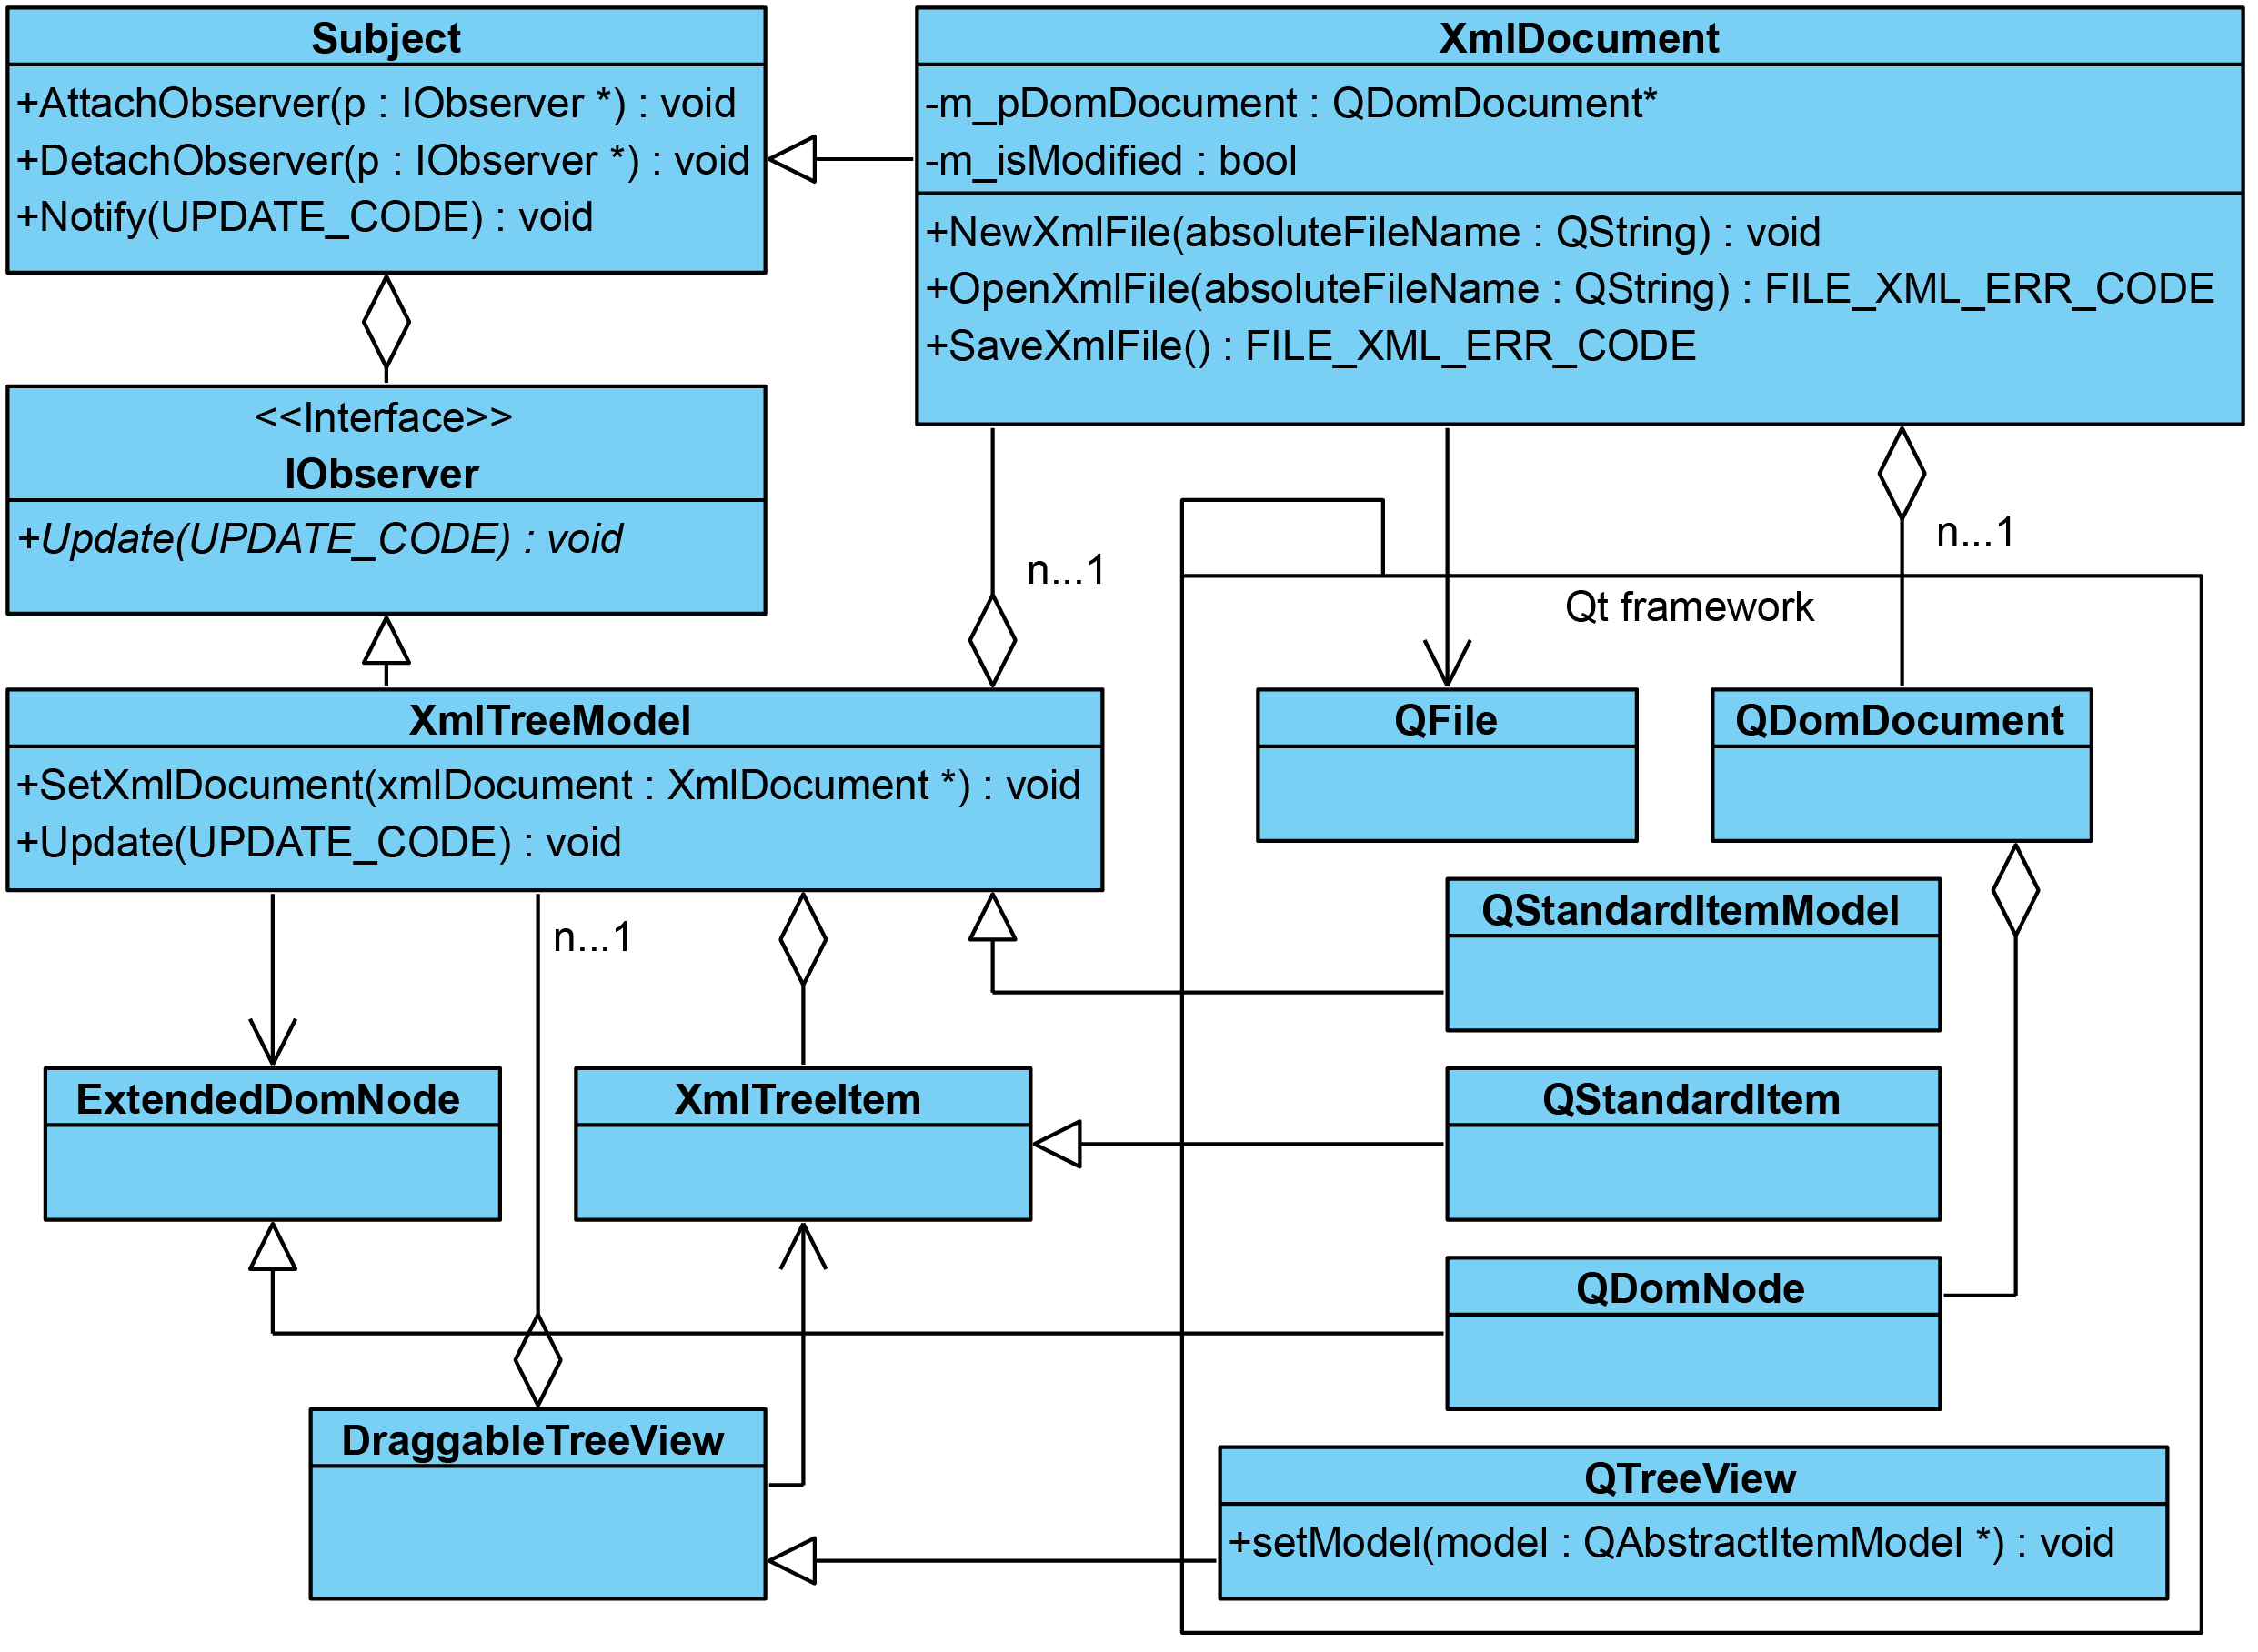
\includegraphics[width=0.98\columnwidth]{tool2/diagramma1.png} 
			\caption{Diagramma dell'integrazione delle classi model-view di Qt\textsuperscript{\textregistered} per la visualizzazione dell'albero XML.}
		\end{figure}
		
		\subsubsection{XML editing diagram}
		In questo diagramma è possibile visualizzare l'implementazione del design pattern \textit{command} usato per gestire l'editing dei file XML. È possibile notare la presenza del design pattern \textit{composite}, inserito allo scopo di permettere la creazione di azioni che si comportassero come singole unità, ma contenessero una aggregazione di azioni base. Un esempio di utilizzo è l'istanziazione automatica di una nuova relazione, la quale crea una singola azione \texttt{XmlEditCommandAggregator} che però esegue tutti i passi intermedi necessari. È a questo punto possibile annullare l'istanziazione con un'unica invocazione del metodo \texttt{Undo} dell'invoker.
		
		\begin{figure}[!h] 
			\centering 
			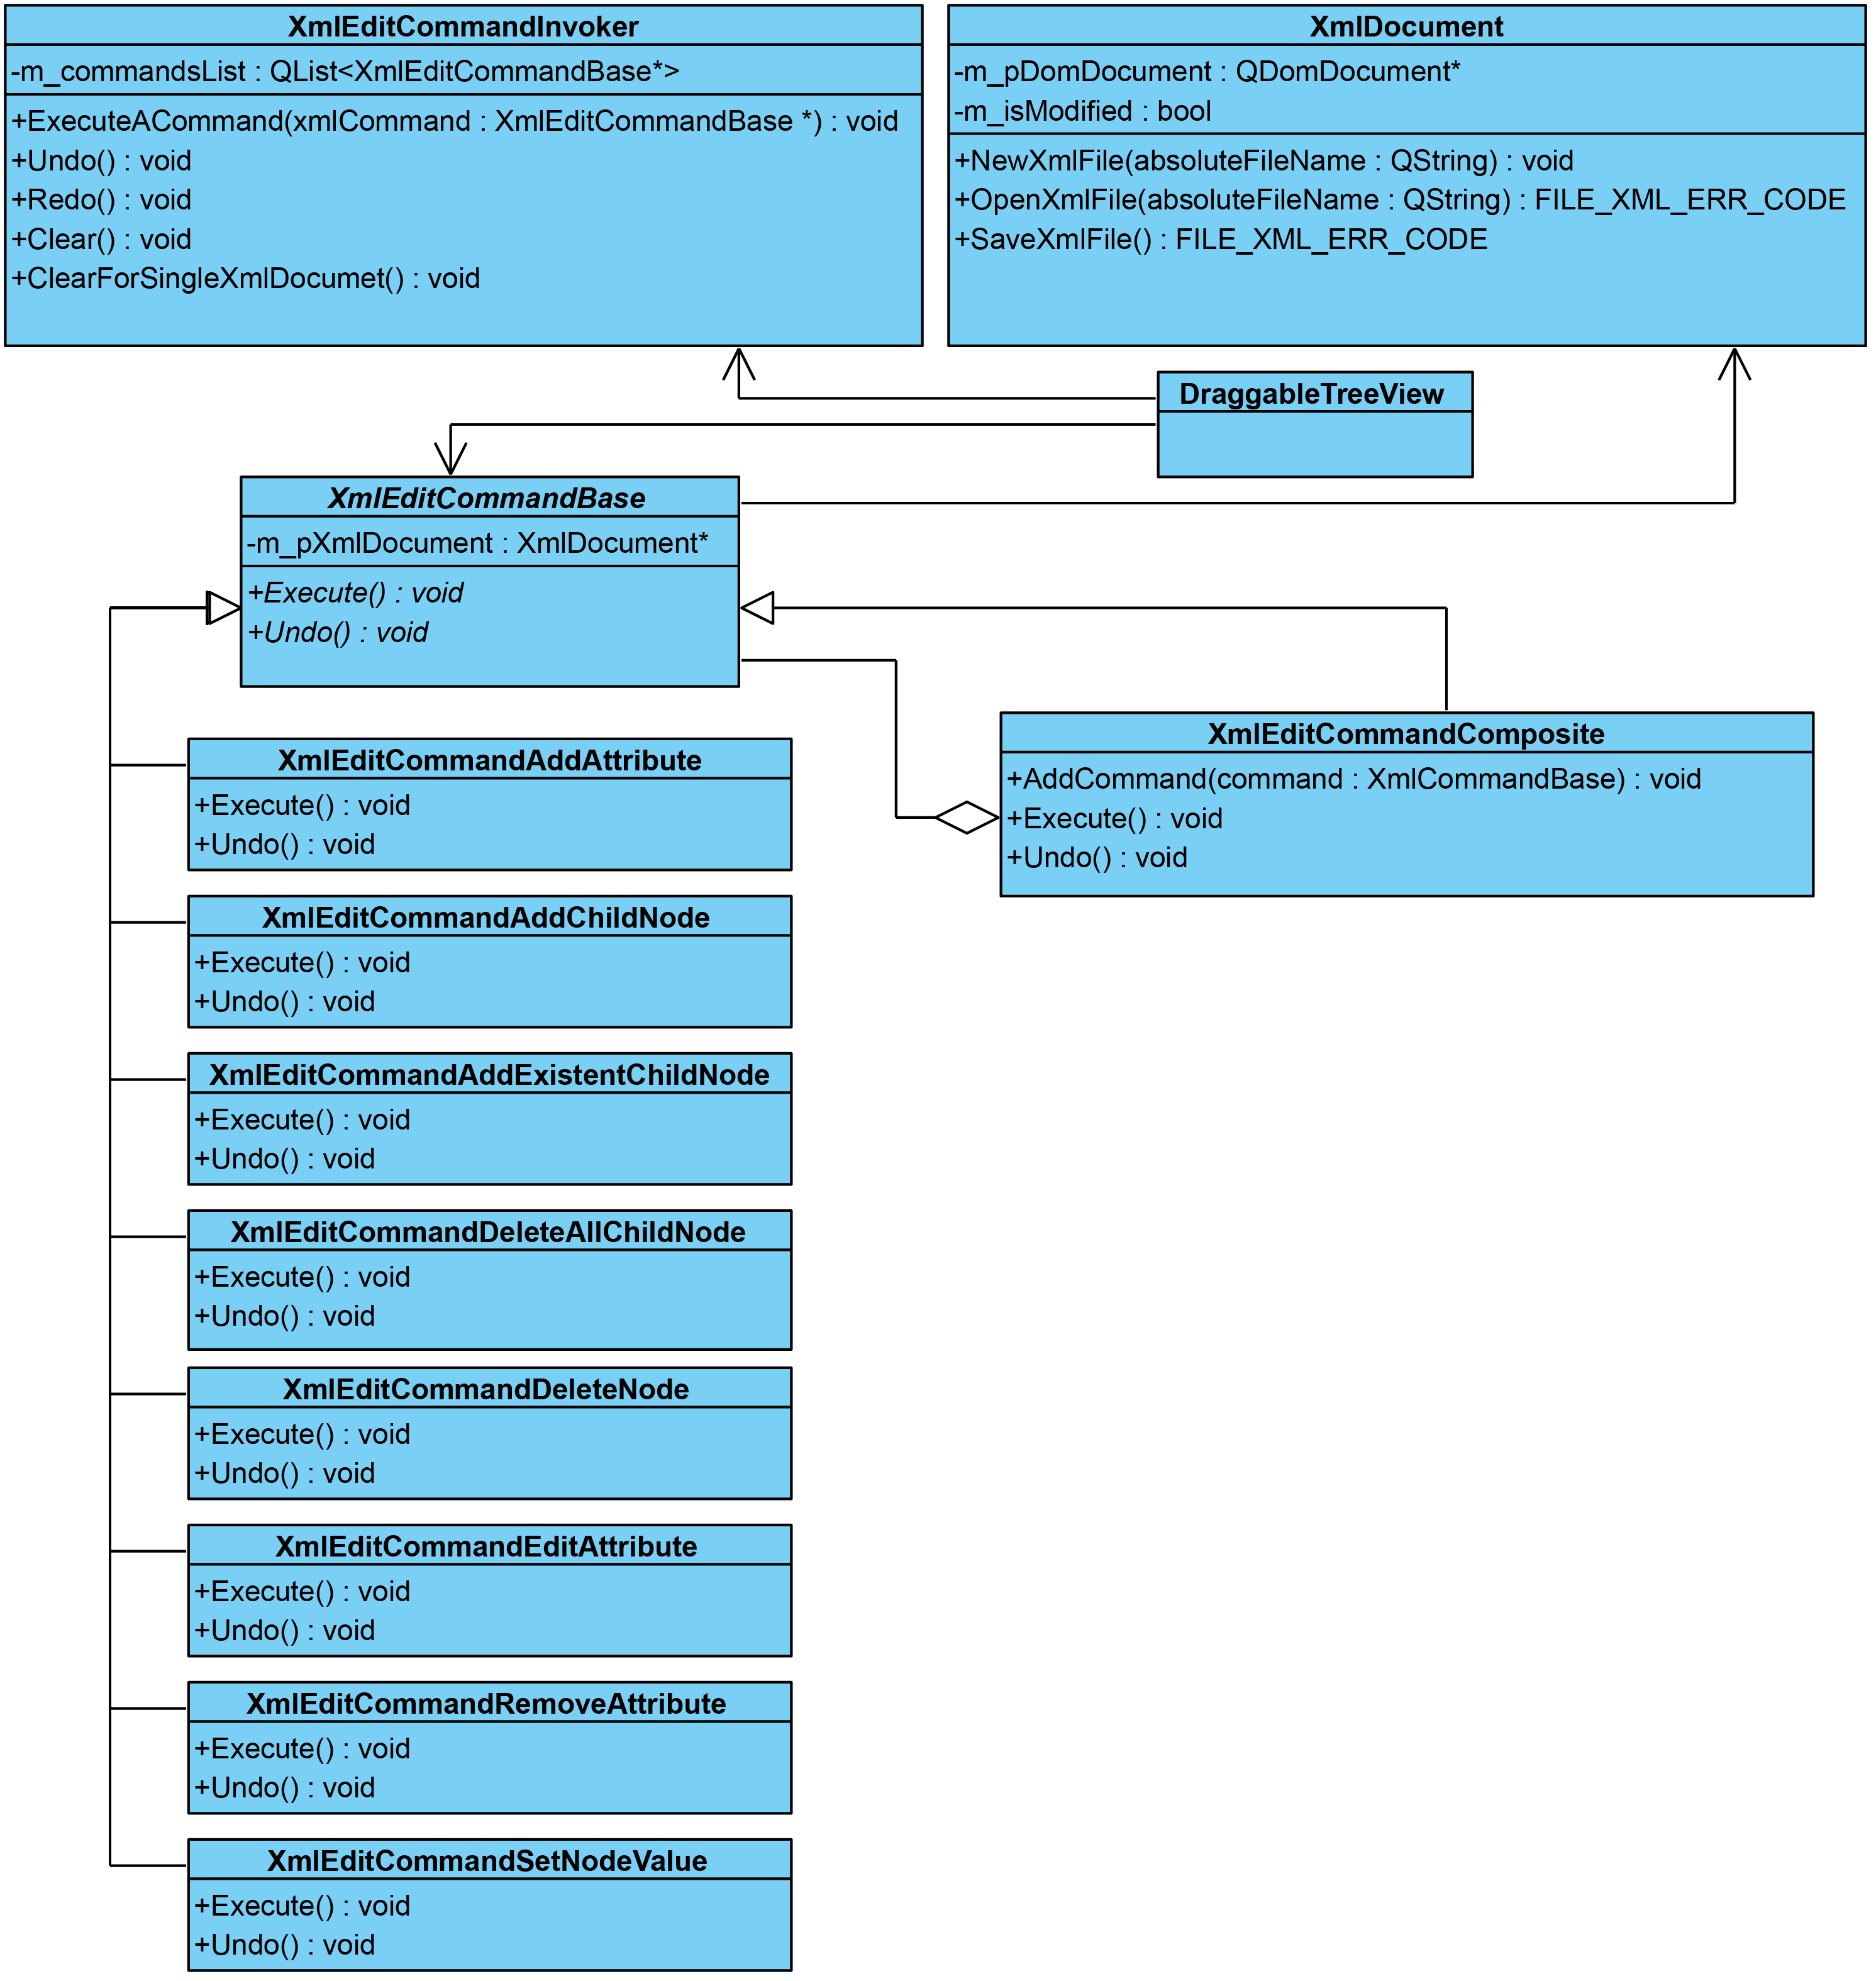
\includegraphics[width=0.98\columnwidth]{tool2/diagramma2.png} 
			\caption{Diagramma delle classi usate per l'editing dei file XML.}
		\end{figure}

\newpage

\subsection{Pacchetto observer}
Questo pacchetto rappresenta l'implementazione del Design Pattern \textit{Observer} ed è stato utilizzato per tenere aggiornata la view al cambiamento dei dati.

	\subsubsection{Interfaccia IObserver}
		\texttt{IObserver} è l'interfaccia che rappresenta gli oggetti che osservano le modifiche di altri oggetti. Essa contiene il metodo virtuale puro \texttt{Update} che i soggetti osservati invocano per segnalare il fatto che sono stati modificati e che quindi un aggiornamento è necessario. Le classi concrete che avranno la necessità di osservare un soggetto deriveranno da \texttt{IObserver} implementando il metodo \texttt{Update}.

	\subsubsection{Classe Subject}
		La classe \texttt{Subject} rappresenta un soggetto che può essere osservato. Essa contiene il codice necessario per notificare tutti gli osservatori dell'avvenuto cambiamento. Mantiene inoltre una lista degli osservatori da notificare, i quali possono iscriversi se desiderano ricevere la notifica, oppure rimuoversi se non è più necessario ricevere aggiornamenti. Le classi che devono essere osservate deriveranno da questa.

\subsection{Pacchetto data}
	Il pacchetto \texttt{data} contiene tutte le classi che rappresentano i dati di business del programma. Come classi aggregazione di base sono state scelte quelle offerte dal framework Qt\textsuperscript{\textregistered} per la loro maggiore integrazione e l'ampio set di funzionalità offerto.

	\subsubsection{Classe AssociatedFiles}
		La classe \texttt{AssociatedFiles} raccoglie tutti i nomi ed i percorsi dei file associati ad un main file. È sua la responsabilità di mantenere la persistenza di queste informazioni tramite la lettura e scrittura nel registro di sistema.
	
	\subsubsection{Classe AttributeNameTagCollapse}
		La classe \texttt{AttributeNameTagCollapse} contiene il filtro sull'attributo da visualizzare nell'albero XML. È sua la responsabilità di mantenere la persistenza di questa informazioni tramite la lettura e scrittura nel registro di sistema.
		
	\subsubsection{Classe XmlDocument}
		La classe \texttt{XmlDocument} rappresenta un file XML aperto nel programma. Ne gestisce la lettura/scrittura su disco e l'effettiva implementazione dell'editing dell'XML.

	\subsubsection{Classe XmlRelation}
		La classe \texttt{XmlRelation} rappresenta un prototipo di relazione, contenendo tutti i dati necessari.
		
	\subsubsection{Classe XmlRelationCollection}
		La classe \texttt{XmlRelationCollection} funge da contenitore per la gestione del set di relazioni cui il programma è a conoscenza.

	\subsubsection{Classe XmlRelationError}
		La classe \texttt{XmlRelationError} rappresenta un errore trovato durante l'analisi di consistenza delle relazioni sulla base dei prototipi conosciuti. Contiene tutte le informazioni dell'errore, le quali saranno mostrate all'utente. È qui presente la logica che compone la stringa descrittiva dell'errore.
		
	\subsubsection{Classe XmlTreeModel}
		La classe \texttt{XmlTreeModel} rappresenta un modello osservabile da una classe view del framework Qt\textsuperscript{\textregistered}. Estende le classi \texttt{QStandardItemModel} e \texttt{Subject}. Essa osserva tramite il pattern \textit{observer} la classe \texttt{XmlDocument} e trasforma il documento XML in un modello visualizzabile dalla classe \texttt{DraggableTreeView}. La classe è un'implementazione del design pattern \textit{Adapter}.
		
	\subsubsection{Classe XmlTreeItem}
		La classe \texttt{XmlTreeItem} estende un classico item del model Qt\textsuperscript{\textregistered} (\texttt{QStandardItem}) inserendo i dati aggiuntivi necessari alla corretta visualizzazione.

\subsection{Core}
	Il pacchetto si occupa della realizzazione dell'analisi e verifica delle relazioni. Utilizza il Design Pattern \textit{Strategy} per l'organizzazione delle classe contenute.

	\subsubsection{Classe XmlRelationCheckerCoreBase}
		\texttt{XmlRelationCheckerCoreBase} rappresenta l'algoritmo di che effettua l'analisi delle relazioni e ritorna una collazione di \texttt{XmlRelationError} con gli errori trovati.
	
	\subsubsection{Classe XmlRelationCheckerCoreImpl}
		La classe \texttt{XmlRelationCheckerCoreImpl} concretizza la base astratta \texttt{XmlRelationCheckerCoreBase} implementando gli algoritmi che effettuano l'analisi dei file verificando la consistenza delle relazioni.

\subsection{Pacchetto command}
Il pacchetto si occupa della gestione delle operazioni di editing dei file XML. Utilizza il Design Pattern \textit{Command} per l'organizzazione delle classe contenute.

	\subsubsection{Classe XmlEditCommandBase}
		\texttt{XmlEditCommandBase} è una classe astratta che rappresenta una operazione eseguibile su un file XML. Mantiene il puntatore al documento XML da editare che verrà usato dalle sottoclassi concrete.
		
	\subsubsection{Classe XmlEditCommandInvoker}
		\texttt{XmlEditCommandInvoker} è la classe che esegue realmente le operazioni mantenendo uno storico di ciò che è stato effettuato offrendo quindi le funzionalità di \texttt{Undo} e \texttt{Redo}

	\subsubsection{Classe XmlEditCommandAggregator}
		\texttt{XmlEditCommandAggregator} è la classe che implementa il design pattern \textit{Command} permettendo l'uso di più comandi come fossero uno singolo.
		
	\subsubsection{Classe XmlEditCommandAddAttribute}
		\texttt{XmlEditCommandAddAttribute} è la classe che implementa il comando di aggiunta di un attributo. Essa mantiene lo stato allo scopo di poter eseguire l'azione di \texttt{Undo}. Per la reale implementazione dell'operazione che essa rappresenta si base sui metodi esposti dalla classe \texttt{XmlDocument}.
		
	\subsubsection{Classe XmlEditCommandAddChildNode}
		\texttt{XmlEditCommandAddChildNode} è la classe che implementa il comando di aggiunta di nuovo nodo vuoto. Essa mantiene lo stato allo scopo di poter eseguire l'azione di \texttt{Undo}. Per la reale implementazione dell'operazione che essa rappresenta si base sui metodi esposti dalla classe \texttt{XmlDocument}.
		
	\subsubsection{Classe XmlEditCommandAddExistentChildNode}
		\texttt{XmlEditCommandAddExistentChildNode} è la classe che implementa il comando di aggiunta di un nodo a partire dalla copia di un nodo precedentemente esistente. Essa mantiene lo stato allo scopo di poter eseguire l'azione di \texttt{Undo}. Per la reale implementazione dell'operazione che essa rappresenta si base sui metodi esposti dalla classe \texttt{XmlDocument}.

	\subsubsection{Classe XmlEditCommandDeleteAllChildNode}
		\texttt{XmlEditCommandDeleteAllChildNode} è la classe che implementa il comando di rimozione di tutti i nodi discendenti di un elemento. Essa mantiene lo stato allo scopo di poter eseguire l'azione di \texttt{Undo}. Per la reale implementazione dell'operazione che essa rappresenta si base sui metodi esposti dalla classe \texttt{XmlDocument}.
			
	\subsubsection{Classe XmlEditCommandDeleteNode}
		\texttt{XmlEditCommandDeleteNode} è la classe che implementa il comando di eliminazione di un attributo e tutti i suoi discendenti. Essa mantiene lo stato allo scopo di poter eseguire l'azione di \texttt{Undo}. Per la reale implementazione dell'operazione che essa rappresenta si base sui metodi esposti dalla classe \texttt{XmlDocument}.
		
	\subsubsection{Classe XmlEditCommandEditAttribute}
		\texttt{XmlEditCommandEditAttribute} è la classe che implementa il comando di editing di un attributo. Essa mantiene lo stato allo scopo di poter eseguire l'azione di \texttt{Undo}. Per la reale implementazione dell'operazione che essa rappresenta si base sui metodi esposti dalla classe \texttt{XmlDocument}.
		
	\subsubsection{Classe XmlEditCommandRemoveAttribute}
		\texttt{XmlEditCommandRemoveAttribute} è la classe che implementa il comando di rimozione di un attributo. Essa mantiene lo stato allo scopo di poter eseguire l'azione di \texttt{Undo}. Per la reale implementazione dell'operazione che essa rappresenta si base sui metodi esposti dalla classe \texttt{XmlDocument}.
		
	\subsubsection{Classe XmlEditCommandSetNodeValue}
		\texttt{XmlEditCommandSetNodeValue} è la classe che implementa il comando di editing del valore di un elemento. Essa mantiene lo stato allo scopo di poter eseguire l'azione di \texttt{Undo}. Per la reale implementazione dell'operazione che essa rappresenta si base sui metodi esposti dalla classe \texttt{XmlDocument}.

\subsection{Pacchetto view}
	Il pacchetto si occupa del display dell'interfaccia utente e della gestione della logica di controllo del software.
	
	\subsubsection{Classe MainWindowView}
		La classe \texttt{MainWindowView} eredita e specializza la classe \texttt{QMainWindow} di Qt\textsuperscript{\textregistered}. Essa è il cuore della logica del programma. Raccoglie e organizza i comandi utente di base, delegando l'esecuzione alle altri componenti del pacchetto.
		
	\subsubsection{Classe DialogAddModifyRelation}
		La classe \texttt{DialogAddModifyRelation} è una dialog creata allo scopo di permettere l'inserimento dei parametri che caratterizzano una relazione da parte dell'utente.
		
	\subsubsection{Classe DialogAssociatedFilesBase}
		La classe \texttt{DialogAssociatedFilesBase} è una base astratta di una finestra di dialog che permette all'utente di gestire i file associati al main file correntemente aperto.
		
	\subsubsection{Classe DialogAssociatedFilesForm}
		La classe \texttt{DialogAssociatedFilesForm} concretizza la base astratta \texttt{DialogAssociatedFilesBase} creando un'interfaccia atta alla gestione dei file associati.
		
	\subsubsection{Classe DialogEditAttributeNameTagCollapseBase}
		La classe \texttt{DialogEditAttributeNameTagCollapseBase} è una base astratta di una finestra di dialog che permette all'utente di gestire il filtro sull'attributo da visualizzare nell'albero XML.
	
	\subsubsection{Classe DialogEditAttributeNameTagCollapse}
		La classe \texttt{DialogEditAttributeNameTagCollapse} concretizza la base astratta \texttt{DialogEditAttributeNameTagCollapseBase} creando un'interfaccia atta alla modifica del filtro sull'attributo da visualizzare nell'albero XML.

	\subsubsection{Classe DialogEditNodeBase}
		La classe \texttt{DialogEditNodeBase} è una base astratta di una finestra di dialog che permette all'utente di editare un nodo XML.
		
	\subsubsection{Classe DialogEditNodeTable}
		La classe \texttt{DialogEditNodeTable} concretizza la base astratta \texttt{DialogEditNodeBase} creando un'interfaccia atta all'editing del valore del nodo e di tutti i suoi attributi.

	\subsubsection{Classe DialogInputFileNameBase}
		La classe \texttt{DialogInputFileNameBase} è una base astratta di una finestra di dialog che permette all'utente di inserire il percorso ed il nome di un file.
	
	\subsubsection{Classe DialogInputFileNameForm}
		La classe \texttt{DialogInputFileNameForm} concretizza la base astratta \texttt{DialogInputFileNameBase} creando un'interfaccia atta all'inserimento di un percorso ed un nome di file. Offre la possibilità di esplorare il file system per un più agevole inserimento. Questa classe è usata per acquisire il file da dove importare o verso dove esportare le relazioni.

	\subsubsection{Classe DialogInputStringBase}
		La classe \texttt{DialogInputStringBase} è una base astratta di una finestra di dialog che permette all'utente di inserire una stringa.
		
	\subsubsection{Classe DialogInputStringForm}
		La classe \texttt{DialogInputStringForm} concretizza la base astratta \texttt{DialogInputStringBase} creando un'interfaccia atta all'inserimento di una stringa da parte dell'utente.
	
	\subsubsection{Classe DialogXmlRelationManagementBase}
	La classe \texttt{DialogXmlRelationManagementBase} è una base astratta di una finestra di dialog che permette all'utente di gestire il database di relazioni.
	
	\subsubsection{Classe DialogXmlRelationManagementTable}
	La classe \texttt{DialogXmlRelationManagementTable} concretizza la base astratta \texttt{DialogXmlRelationManagementBase} creando un'interfaccia atta alla gestione delle relazioni, visualizzate sotto forma tabellare.

	\subsubsection{Classe ViewXmlRelationErrorsBase}
		La classe \texttt{ViewXmlRelationErrorsBase} è una base astratta di una finestra di dialog che permette all'utente di visualizzare il risultato del controllo di consistenza delle relazioni.
		
	\subsubsection{Classe ViewXmlRelationErrorsTable}
		La classe \texttt{ViewXmlRelationErrorsTable} concretizza la base astratta \texttt{ViewXmlRelationErrorsBase} creando un'interfaccia tabellare per la visualizzazione dei risultati sul check delle relazioni.

	\subsubsection{Classe DraggableTreeView}
		La classe \texttt{DraggableTreeView} deriva dalla classe \texttt{QTreeView} del framework Qt\textsuperscript{\textregistered}. Essa è quindi in grado di visualizzare la classe model \texttt{XmlTreeModel} nella quale abilita il drag \& drop per l'istanziazione automatica. È sua responsabilità l'invocazione dei command tramite l'invoker.
	
	
	\subsubsection{Classe XmlViewBase}
		La classe \texttt{XmlViewBase} è una base astratta di un widget per la visualizzazione di file XML.
	
	\subsubsection{Classe XmlViewTree}
		La classe \texttt{XmlViewTree} concretizza la base astratta \texttt{XmlViewBase} creando un widget che mostra un file XML sotto forma di albero.

\section{Codifica}
Tutto il codice del tool è stato pubblicato sulla piattaforma GitHub\textsuperscript{\textregistered}, accedibile tramite il seguente indirizzo: \url{https://github.com/Mauxx91/XML-Editor}. Tutto il codice è disponibile gratuitamente sotto licenza GNU GPL v3\footnote{Un approfondimento sulla licenza può essere trovato al seguente indirizzo: \url{http://www.gnu.org/copyleft/gpl.html}.}\\

Tutto il codice è stato scritto in lingua inglese, compresi i commenti, dei quali si è cercato di scriverne il più possibile.
La codifica ha seguito alcune convenzioni della famosa notazione Ungherese. Di seguito sono elencati i formalismi utilizzati nel codice:

\begin{itemize}
	\item \textbf{prefissi:}
	\begin{itemize}
		\item \textbf{m}: usato per le variabili membro (esempio: \texttt{m\_keyName});
		\item \textbf{p}: usato per le variabili puntatore (esempio: \texttt{m\_pkeyNameList});
		\item \textbf{o}: usato per le variabili input alla funzione che sono usate come output (esempio: \texttt{o\_foundKeys});
		\item \textbf{I}: usato per le classi interfacce (esempio: \texttt{IObserver}).
	\end{itemize}
	\item \textbf{suffissi:}
	\begin{itemize}
		\item \textbf{Base}: usato per le classi astratte (esempio: \texttt{ResultWidgetBase});
	\end{itemize}
	\item \textbf{capitalizzazione:}
	\begin{itemize}
		\item \textbf{variabili e parametri}: iniziano sempre in minuscolo e usano una lettera minuscola per ogni parola (esempio: \texttt{m\_parentWidget}, \texttt{returnValue});
		\item \textbf{macro ed enum}: completamente in maiuscolo con le diverse parole separate dal carattere \sq{\_} (esempio: \texttt{UPDATE\_CODE});
		\item \textbf{classi, funzioni e metodi}: iniziano sempre in maiuscolo e ogni parola diversa parte in maiuscolo (esempio: \texttt{FileOccurrence});
	\end{itemize}
\end{itemize}

\section{Conclusioni}
Tutti i requisiti sono stati soddisfatti come pianificato ma, il secondo incremento comprendente le funzionalità di editing è stata completata con 10 ore di ritardo sulla pianificazione iniziale. 
la realizzazione di questo tool ha permesso allo studente di conoscere davvero approfonditamente il framework Qt\textsuperscript{\textregistered} ed implementare un tool di buona utilità anche all'esterno dell'azienda. L'utilizzo del nuovo design pattern architetturale model-view si è rivelato davvero adatto allo sviluppo di sistemi di questa tipologia, dimostrandosi una valida alternativa a MVC.
